\documentclass[letterpaper]{article} % DO NOT CHANGE THIS
\usepackage[submission]{aaai2027}  % DO NOT CHANGE THIS
\usepackage[hyphens]{url}  % DO NOT CHANGE THIS
\usepackage{graphicx} % DO NOT CHANGE THIS
\urlstyle{rm} % DO NOT CHANGE THIS
\def\UrlFont{\rm}  % DO NOT CHANGE THIS
\usepackage{natbib}  % DO NOT CHANGE THIS AND DO NOT ADD ANY OPTIONS TO IT
\usepackage{caption} % DO NOT CHANGE THIS AND DO NOT ADD ANY OPTIONS TO IT
\frenchspacing  % DO NOT CHANGE THIS
\usepackage{booktabs}
\usepackage{amsmath,amssymb}
\pdfinfo{
/TemplateVersion (2027.1)
}
\setcounter{secnumdepth}{2}

\newcommand{\SWT}{stratified Wald-t limit}
\newcommand{\SWL}{stratified Wilson-type limit}
\newcommand{\NSF}{\textsc{nsf}}

\title{Certifying a Language-Model Update Before Release:\\What Holds, What a Label Buys, and What Does Not Carry}
\author{Anonymous Submission}
\affiliations{}

\begin{document}

\maketitle

\begin{abstract}
Before an updated language-model policy is released, a developer wants a statement such as ``this model refuses at
most 5\% of benign requests'' that is wrong with a small stated probability. The safety test of a Seldonian algorithm
gives such a certificate from labelled responses that played no part in choosing the update. We test, where the true
rate is known, when it can be trusted. Exact binomial bounds kept their promise on data sampled as they assume. The
normal limits shipped with two published ways of letting an automatic judge stand in for labels did not at safety-test
sizes: in our implementation the first was wrong in 6\% to 11\% of trials at a promised 5\% at a 20\% rate, both in up
to 24\% at a 1.3\% rate. Grouping
prompts by how often the model before the update showed the behaviour made a label worth 1.3 to 1.5 labels on new prompts
at rates of 12\% and 46\% (the second from a pool mixed from two sources), under an approximate limit; it gained little or
lost at 82\% and above and at rare rates, and almost nothing once the update reordered the prompts. Across the update, a
rubric judge's error rates did not carry in any of three seeds of one set-up, while a second judge's did. On a crossed
agent benchmark, bounds that treat task pairs as independent failed for 27 of 28 agents; with the attacks taken as
fixed, one certifies a 5\% attack success rate under an approximate bound. One annotator's labels give an exact bound
of 20.1\% on a trained policy's outright refusals, but do not certify the 2-point limit on their change that it was
trained under.
\end{abstract}

\section{Introduction}

A policy update is a release decision. After further training, a developer who ships the new model is implicitly
claiming that some unwanted behaviour (a needless refusal, a harmful answer, a successful prompt injection) has not
become more frequent than a stated limit. Reported rates do not make that claim; a regression gate does. We call a
statement ``the rate is at most $\tau$'', made by a procedure that is wrong with probability at most $\delta$, a
\emph{certificate}, and the procedure that produces it a release gate for the update.

The Seldonian framework \citep{thomas2019preventing} builds this gate into learning. Data are split into a candidate
set and a safety set; any search on the candidate set proposes one updated policy; a one-sided upper confidence bound
on each constrained rate, computed once on the sealed safety set, decides whether the policy is returned or the answer
is ``no solution found'' (\NSF{}). Because the candidate is fixed before the safety set is read, the gate is valid for
any training procedure, including reinforcement learning on a reward the constraint does not measure.

Three features of language-model evaluation can void that guarantee without any visible sign. The label is not
observed: a guard model, a rubric judge or a benchmark harness produces it, and its errors can differ between the
model before and after the update. The sample is often not independent: agent benchmarks cross tasks with attacks.
And the rates of interest are small, where normal approximations fail \citep{bowyer2025clt}. This paper does not propose
a training method. It takes the safety test as a release gate for an updated policy and asks, where the truth is known,
which bounds keep their promise, what a label budget buys, and what does not carry from the model before the update to
the model after it. Our findings:
\begin{enumerate}
\item \textbf{Which bounds hold} (Section~\ref{sec:valid}). Exact bounds held on data sampled as they assume. The
  normal limits of judge-assisted estimators, PPI++ and StratPPI, ran over their level at safety-test sizes. With a
  bootstrap-t limit and labels allocated in proportion to stratum size, the same estimators held in the cells we first
  ran, partly by declining to certify; on new prompts StratPPI's was over in 2 of 32 refusal-label cells (one at 82\%, one
  at 98\%; for a claim about the prompt source it was over in most cells), and under its paper's own
  allocations it failed.
\item \textbf{What a label buys} (Section~\ref{sec:strata}). Strata built from the pre-update model's own per-prompt
  rate are fixed before the update, so the update can cost them width but not the sampling design's validity; with the
  \SWT{} (a Student-t limit on the stratified estimate) they stayed valid in the one run that reordered the prompts. Their gain is modest, confined to mid
  rates (we saw gains from 9\% to 66\%, little or none at 82\% and above or under 4\%) and to an approximate limit, and disappears when the update reorders the prompts.
\item \textbf{What does not carry across an update} (Section~\ref{sec:carry}). A judge's measured error rates across
  prompt populations, and a rubric judge's across training that targets the judged label (a second judge's carried);
  and independent-sample bounds on a crossed agent benchmark.
\end{enumerate}
Section~\ref{sec:human} gives the one certificate in human labels we can compute, and its cost. Many of the results
were checked against predictions committed before their runs: of 72, 53 held, 18 failed and one could not be tested;
leaving out five that say only that an exact bound is exact and ten written after a dry run, 39 of 57 held
(Appendix~\ref{app:record}).

\section{The Gate and How We Check It}
\label{sec:setup}

\paragraph{The safety test.} Let $\pi_\theta$ be a policy, $x$ a prompt, $y\sim\pi_\theta(\cdot\mid x)$ a response and
$c(x,y)\in\{0,1\}$ a label from a judge (a guard model, a rubric judge, code, or a human), with $1$ meaning the unwanted
event. The \emph{behaviour rate} is $p(\theta)=\mathbb{E}_x\mathbb{E}_y[c(x,y)]$ over a prompt population. A
constraint is absolute, $p(\theta)\le\tau$, or relative to the policy before the update, $p(\theta)-p(\theta_0)\le m$.
After training, one candidate $\theta_c$ is selected; on $n_s$ safety prompts it never saw, one response each is drawn
and labelled, and an upper limit $U$ at level $\delta$ is computed. The gate returns $\theta_c$ if $U\le\tau$ and
\NSF{} otherwise. A bound is \emph{valid} if $P(U<p)\le\delta$ for a fixed policy and an independent sample; given the
candidate set, $\theta_c$ is fixed, so $P(\text{returned and }p(\theta_c)>\tau)\le\delta$ for any selection rule
\citep{thomas2019preventing}. Declining is always allowed, so the rate at which the gate passes is part of the result.
In the training runs we use, a relative threshold was set once from the pre-update model's rate on
candidate prompts plus the margin, and then treated as a constant; their gate certifies the rate against that number, not
the difference itself, which Section~\ref{sec:human} bounds. A gate that only approximates the guarantee, through an
approximate bound, is \emph{quasi-Seldonian} \citep{thomas2019preventing}.

\paragraph{Measuring validity.} Validity is one number per setting, the \emph{miss rate} $P_S(U(S)<p)$ over draws of
the sample $S$. It cannot be read off one real sample, so we compute it where $p$ is known, in three ways: (i)
\emph{resampling real responses} \citep{franklin2014plasmode}, where a pool of labelled responses is the population and
its mean the truth (pools of 400 to 500 prompts, benign ones from XSTest
\citep{rottger2024xstest} and OR-Bench \citep{cui2025orbench} and harmful ones from PKU-SafeRLHF \citep{ji2025pkusaferlhf},
plain or encoded, and OR-Bench's toxic set, with 8 or more responses per prompt from the model before and after an update; Granite-3.3-2B \citep{granite2025} and Qwen2.5-1.5B-Instruct \citep{qwen25}, labelled by
Qwen3Guard-4B \citep{qwen3guard2025}); (ii) a synthetic contextual bandit on which our training code runs unchanged and
every policy's rate is exact; and (iii) resampling the published tables of a crossed benchmark. Every bound is scored
by one rule: with $R\ge4{,}000$ draws and $se=\sqrt{\delta(1-\delta)/R}$, a cell is \emph{over} its level if the miss
rate exceeds $\delta+2se$, \emph{unresolved} if it lies between $\delta$ and $\delta+2se$, and at or under otherwise.
Each row of the full table (Appendix~\ref{app:validity}) also reports the largest upper end of a 95\% interval for a
cell's miss rate and the cells still over after a Bonferroni correction. As in our registrations, a \emph{mid-rate}
label is one between 5\% and 95\%.

\paragraph{The bounds.} Clopper-Pearson \citep{clopper1934} and the betting bound of \citet{waudbysmith2024betting} are
exact. Student's t and Wilson's score bound are approximate. For a sample stratified into strata $h$ with shares
$W_h$, $n_h$ labels and rates $\hat p_h$, the \SWT{} is
$\hat\mu+t\sqrt{\sum_h W_h^2\tilde p_h(1-\tilde p_h)/(n_h-1)}$ with $\hat\mu=\sum_hW_h\hat p_h$, smoothed rates
$\tilde p_h$ and Satterthwaite's degrees of freedom; the \SWL{} puts the variance at the hypothesised rate instead. A
judge enters through PPI++ \citep{angelopoulos2023ppipp}, which corrects the labels' mean by the judge's score on many
unlabelled responses, or StratPPI \citep{fisch2024stratppi}, which does so within strata; both ship with a normal limit,
and we also pair them with a studentised bootstrap (bootstrap-t) limit \citep{hall1988}; PPBoot \citep{zrnic2024ppboot}
uses a percentile bootstrap instead. Clustered data use a cluster
bootstrap-t. Appendix~\ref{app:defs} gives every formula. We compare widths by an effective sample size,
$\mathrm{ESS}=(w_{\text{base}}/w_A)^2$, where $w$ is the mean distance from the truth to the limit and the baseline is a
random sample of the same size with a pooled bound: an ESS of 2 means $n$ labels do the work of $2n$.

\section{Which Bounds Hold}
\label{sec:valid}

Table~\ref{tab:valid} condenses the validity table of Appendix~\ref{app:validity} (55 rows); the confirmation pools,
the routing rule and the judge-assisted exact bounds are reported in Appendices~\ref{app:strata} and~\ref{app:judge}.
Four readings follow.

\begin{table}[t]
\centering
\small
\setlength{\tabcolsep}{3pt}
\begin{tabular}{@{}p{3.9cm}rr@{}}
\toprule
bound (setting, $\delta$) & over / cells & worst miss \\
\midrule
\multicolumn{3}{@{}l}{\emph{exact}} \\
Clopper-Pearson (judge pools, 0.05) & 0 / 42 & 0.052 \\
Clopper-Pearson, random draws (0.05) & 0 / 28 & 0.050 \\
\multicolumn{3}{@{}l}{\emph{approximate, not over in these cells}} \\
PPI++, bootstrap-t limit (0.05) & 0 / 168 & 0.054 \\
StratPPI estimator, bootstrap-t, proportional (0.05) & 0 / 56 & 0.056 \\
\SWT{}, 8 strata of the pre-update rate (0.05) & 0 / 28 & 0.036 \\
the same, redrawn with replacement (0.05) & 0 / 28 & 0.038 \\
cluster bootstrap-t by user task, AgentDojo (0.05) & 0 / 28 & 0.051 \\
\multicolumn{3}{@{}l}{\emph{over its level}} \\
PPI++, normal limit (0.05) & 126 / 168 & 0.241 \\
StratPPI, normal limit, proportional (0.05) & 35 / 56 & 0.239 \\
StratPPI, normal limit, heuristic allocation (0.05) & 24 / 28 & 0.90 \\
PPBoot, percentile limit (0.05) & 19 / 28 & 0.148 \\
\SWL{}, redrawn with replacement (0.05) & 7 / 28 & 0.062 \\
\SWT{}, synthetic i.i.d.\ grid (0.05) & 5 / 18 & 0.111 \\
Clopper-Pearson over pairs, AgentDojo (0.05) & 27 / 28 & 0.268 \\
\bottomrule
\end{tabular}
\caption{Miss rates against $\delta$, condensed from Appendix~\ref{app:validity}. A cell is one bound, design,
population, sample size and $\delta$, with 4{,}000 to 40{,}000 draws; ``over'' is Section~\ref{sec:setup}'s rule. The
bootstrap-t rows hold partly by returning no limit (see text).}
\label{tab:valid}
\end{table}

\paragraph{Exact bounds held where their assumptions hold.} No exact bound was over its level on data sampled as it
assumes. The t-test is the wrong default for a rate: by enumeration over binomial counts, the Student-t limit's miss
probability is above $\delta$ at 96\% or more of 79 rates from 0.5\% to 20\%, at each of five sample sizes from 200 to
2,400 and at $\delta$ of 0.05 and 0.10, and Clopper-Pearson's is above it at none. The t limit's width is zero when no positive
is seen: a policy with a true rate of 1\% passes a 0.5\% threshold whenever 100 samples hold no positive, which is 37\%
of the time. Wilson's bound is not safe at the edges either: just above the limit it returns with no positive its miss
is 0.069 at $n=100$ and $\delta=0.05$, and just under a rate of 1 it reaches 0.20.

\paragraph{Judge-assisted normal limits did not hold at safety-test sizes.} With 225 labels at a 1.3\% rate, PPI++
with its normal limit missed in up to 24\% of draws at $\delta=0.05$; at a 20\% rate and 100 to 500 labels it missed in
6\% to 11\%. StratPPI as published, with labels stratified on a rubric judge's logit, was over its level in 26 of 28
cells under proportional allocation. Under the heuristic allocation of its paper one cell missed in 90\% of draws:
four strata where the judge's probability is under 0.001 keep 2 labels each, the minimum we set, see no positive in
91\% of draws, and drop a fifth of the rate (with a minimum of 10 labels a stratum the cell still misses in 59\%). These
are finite-sample findings in our implementation and do not contradict the methods' asymptotic guarantees. PPI++ with
a bootstrap-t limit, and StratPPI's estimator with one under proportional allocation, were over their level in none of
168 and 56 cells.
Part of that record is abstention: a bound that returns no limit cannot miss, and counted as misses instead, those
returns would put up to 7 of 28 cells of one row over.

\paragraph{Judge-assisted exact bounds bought nothing.} Finite-sample judge-assisted bounds (betting bounds on blocks
of judged responses) were
valid and narrower than the labels alone in 10 of 84 cells, by at most 0.003. Reporting the smaller of Clopper-Pearson
on the labels and the PPI++ bootstrap-t limit is not a bound: it missed in up to 0.078 of draws at $\delta=0.05$. A fixed routing rule avoids that choice. Code
computes any property code can verify; with fewer than 10 gold labels in the rarer class, Clopper-Pearson on the labels;
with 10 or more, PPI++ on the judge's logit with a bootstrap-t limit; a calibration measured on another population is
refused (Table~\ref{tab:routing}; for a stratified
sheet, the caution about the Wilson-type limit below applies). Resampled as one procedure, the rule missed in at most 0.052 of draws over 20 cells,
none over its level. The rule and its threshold were settled on these results, not before them.

\paragraph{``Approximate'' carries a number.} Over the first 36 rows of the full table, leaving out the bounds marked as
failing, no cell stays over its level after the correction, and the largest miss a cell's interval leaves open is 0.067
at $\delta=0.05$; of the registered rows that follow, three non-failing bounds have 1 to 3 cells over (interval ends up
to 0.062 at $\delta=0.05$). In
the designs they were run in, the approximate bounds we use were over their level in 1 of 378 cells (a grouping made
after the results), but that depends on the design: the \SWL{} kept its level when the safety set was 20--40\% of a
finite pool and was over in 7 of 28 cells once the pool was large, all at rates of 65\% and above, and the \SWT{} is
over in 5 of 18 cells on a synthetic i.i.d.\ grid. An approximate limit with a good record here is still a
quasi-Seldonian gate.

Selection does not break a valid gate. Inside our training loop on the synthetic bandit (Lagrangian GRPO
\citep{shao2024grpo}, 8 strata, 8,000 runs a cell), the \SWT{} for the pool's own rate was over its level in none of 8
cells; with the term for a sampled pool, for the population's rate, it was over in 2 of 8, both in the least
heterogeneous environment (Appendix~\ref{app:pipeline}). In a classifier setting, rerandomised and stratified
candidate/safety splits, including candidates built to overfit the balancing statistics, did not break an exact test in
2,000 seeds per arm, nor a tight Wald test sensitive enough to show a leak (misses at most 0.055 at $\delta=0.05$).

\section{What a Label Buys: Strata from the Model Before the Update}
\label{sec:strata}

A relative constraint already calls for the pre-update model's responses, so they can also shape the safety sample. Draw
$k=8$ responses of the pre-update model to every prompt in the pool, rank the prompts by the share the judge flags, cut
the ranking into 8 equal strata with ties broken at random, and draw the safety set within strata in proportion to their
size. The strata use no response of the updated policy and are fixed before the safety set is drawn, so the update can
cost them width but not validity. They remove the between-stratum share $G$ of the variance, an ESS of about $1/(1-G)$,
which a pre-flight formula predicts from the pre-update samples (Appendix~\ref{app:defs}).

\paragraph{Confirmation on new prompts.} The strata rule and the limits were chosen on the pools that measured them,
where the \SWL{} gained 1.4 to 5.1 at rates of 9\% to 66\% (ESS from the truth, redrawn with replacement; the upper end
on a label where it is over its level). We therefore registered predictions and tested them on new prompts: three pools of
400 OR-Bench prompts \citep{cui2025orbench} answered by a Granite-3.3-2B policy trained under a relative over-refusal
constraint (refusal rates 12\%, 82\% and 98\%), a fourth pool mixed to land at a mid rate (46\%; weaker evidence: a rate we aimed at, predictions written after a dry
run, and two prompt sources that the strata largely separate, which alone remove about three quarters of the variance
the strata remove), a second model family
(Qwen2.5-1.5B-Instruct at 19\%), and the same family after an update that moved it far from its reference (58\%; the
correlation of reference and trained per-prompt rates was 0.46, against 0.84 after the update that kept the order).
Table~\ref{tab:strata} gives the gains of the \SWT{}, which for the pool's own rate was over its level in no mid-rate
cell of these pools; a claim about the prompt source the pool was drawn from adds a term for the pool's own sampling
error, and with it the limit was over in 1 of 8 cells on the second family. On the human labels of the last row it
was over in 3 of 64 cells, by at most 0.008.

\begin{table}[t]
\centering
\small
\setlength{\tabcolsep}{3.5pt}
\begin{tabular}{@{}p{3.65cm}cc@{}}
\toprule
pool (refusal rate) & pool's own rate & prompt source \\
\midrule
Granite, new prompts (12\%) & 1.47, 1.73 & 1.31, 1.32 \\
Granite, mixed pool (46\%) & 2.09, 2.56 & 1.49, 1.34 \\
Granite, new prompts (82\%) & 0.86, 1.13 & 0.75, 0.89 \\
Granite, new prompts (98\%) & lost (all limits) & 0.11, 0.25 \\
Granite, rare (1.6--3.2\%) & 0.86--1.20 & 0.85--1.13 \\
Qwen, order kept (19\%) & 1.52, 1.77 & 1.35, 1.35 \\
Qwen, reordered (58\%) & 0.97, 1.08 & 0.94, 0.97 \\
human labels (6--60\%) & 1.18 (median) & not run \\
\bottomrule
\end{tabular}
\caption{ESS of the \SWT{} with 8 reference-rate strata, at safety sets of 100 and 200, against a random draw with a
pooled Wilson bound; $\delta=0.05$. Pool's own rate: drawn with replacement within strata; prompt source: the pool
redrawn and the strata rebuilt, 10,000 replications. Last row: XSTest's human labels of five released
models, strata from another model's guard rate, eight mid-rate labels (two definitions on five models)
at 6\% to 60\%, safety set 100. Rare: two labels
from the guard's safety field. Full results in Appendix~\ref{app:strata}.}
\label{tab:strata}
\end{table}

Four things follow. \emph{The gain is modest and confined to moderate rates.} For a certificate about the prompt source it
was 1.3 to 1.5 at 12\% and 46\%; at 82\% and above, and on rare labels, the strata gained little or lost, and on rare
labels an exact bound on a random draw is the one to use. \emph{It depends on the update keeping the order of
prompts.} Where training kept the pre-update order, the gain survived; where it reordered the prompts, the limit stayed
valid and the gain went to 0.97 and 1.08, which the pre-flight from pre-update samples alone did not foresee (it
predicted 1.55). \emph{It belongs to the approximate limit.} Two exact stratified bounds kept their level in all 116
cells we drew, but neither gave a gain to rely on: a stratified Clopper-Pearson bound certified more often than
Clopper-Pearson on a random draw of the same size in 19 of 36 real-response cells and in none of 32 cells on human
labels, at the threshold we registered, and a stratified betting bound never did. \emph{It pays only where the certified label is costly.} The strata
cost 8 judged pre-update responses per prompt. When the certified label is itself a human one, a gain of about 1.2
saves about 17 of 100 labels for 2,000 judged responses (8 for each of 250 prompts), which pays where a human label
costs more than about 120 judged responses; the break-even grows with the pool. Where strata and label come from the same cheap judge, a larger safety set is the better use of the budget.

\paragraph{Predicting the gain before labelling.} The pre-flight ranks the gain well (Spearman 0.84 between predicted and
realised ESS over 432 cells, ESS from the estimate at $\delta=0.10$, with the updated policy's quantities measured) and
over-predicts its size. On the new prompts, with the updated policy's two quantities
measured on responses the draws do not use, it was within 20\% of the \SWL{}'s gain at 12\%, 46\% and 82\%; from the pre-update samples alone
it predicted 2.58, 4.12 and 2.22, and the realised gains of the \SWL{} were 27\% to 41\% lower. A gate planned before the update should
therefore budget for the gain of a random sample.

\paragraph{Against StratPPI.} On the same strata and draws, StratPPI's published limit is shorter partly because its
normal limit runs over its level (in 9 of 28 cells counted by checkpoint). With a bootstrap-t limit and proportional
allocation its estimator holds and gains about as much (median ESS 2.10 against 2.16 for the \SWL{}); at a safety set of
100 with 8 strata the regression on the reference rate within strata adds nothing once the limit is valid
(Appendix~\ref{app:strata}).

\section{What Does Not Carry Across an Update}
\label{sec:carry}

\subsection{A judge's measured error rates}

The cheapest gate uses no gold label on the updated policy: measure the judge's recall $r$ and false-alarm rate $f$ on
labelled responses of the pre-update model, measure its flag rate $q$ on the updated policy, and bound
$p=(q-f)/(r-f)$ \citep{rogan1978} from one-sided limits on the three. It is valid only if $r$ and $f$ are the same on
both sides of the update. We tested this \emph{carried} bound for a judge compiled from a one-sentence rubric (Qwen3-8B
scoring each response by its probability of answering Yes, six wordings of the rubric), with the guard's refusal flag as
gold (Figure~\ref{fig:carry}).

\begin{figure}[t]
\centering
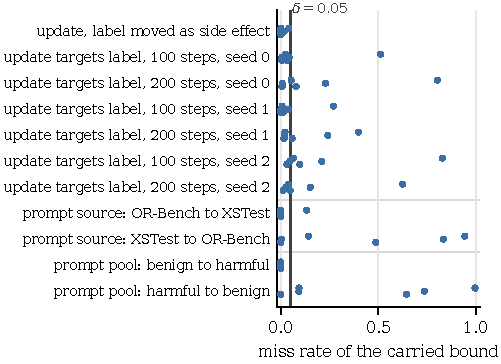
\includegraphics[width=\columnwidth]{fig_carry.pdf}
\caption{Miss rate of a carried calibration at $\delta=0.05$, one dot per rubric wording. Top seven rows: the judge
calibrated on the model before an update and applied after it; the run that targets the label has three seeds. Bottom
four: calibrated on one prompt population and applied to another.}
\label{fig:carry}
\end{figure}

\paragraph{Across prompt populations} the carried bound missed in up to 94\% of draws between two sources of benign
prompts and in up to 99.6\% between benign and harmful pools. The failure depends on direction; between the pools, in
the direction where it was over for no wording, it returned no certificate in at least 98\% of draws.

\paragraph{Across an update.} A calibration did carry across 200 steps of a run (one seed) that moved the label
only as a side effect: recall differed in none of six wordings (under two of them the carried bound returned no certificate in 90\%
and 77\% of draws). It did not carry across a run whose Lagrangian penalised the judged
label (GRPO with LoRA on Granite-3.3-2B, a relative over-refusal constraint), in any of three seeds: the canonical
wording's recall on the guard's refusals fell from 0.21 to 0.03, 0.07 and 0.05, and the carried bound was over its level
for 3, 3 and 2 of six wordings (misses up to 0.80), although the pool's refusal rate stayed within 1.4 points of the
pre-update model's. The predictions for seeds 1 and 2 were registered before they were trained, and all held; one seed was retried after a
crash without the explicit decision the registration reserved (Appendix~\ref{app:record}).

A second judge behaved differently, against our registered prediction that it too would fail. WildGuard
\citep{han2024wildguard}, scored on the same
4,500 responses, kept its recall on the guard's refusals across the update (0.88 before; 0.94, 0.94 and 0.91 after), and
its carried bound was over its level in no seed; with WildGuard as gold, the compiled judge's carried bound failed in all
three. Against one annotator's labels the direction is the same, without significance: the compiled judge flags 3 of 18
strict refusals before the update and 0 of 18 after, while the guard's recall does not move (17 and 16 of 18). Our
account, which no experiment isolates, is a change in form: after training, the guard's flags are mostly long refusals
with a helpful-sounding body (29 of 100 guard flags before; 83 of 93, 83 of 108 and 85 of 97 after, by seed), which the
rubric judge reads as answers,
and the judge also read plain refusals differently after training (Appendix~\ref{app:judge}). WildGuard also began with far higher recall (0.88 against 0.21), so the failure may
belong to weak judges rather than rubric judges; with one judge of each kind we cannot say which. Reading the
side-effect run as a control came after the result. For a release gate the rule is plain: gold labels belong on
the responses of the updated policy, each time it is updated.

\subsection{Independent-sample bounds on a crossed agent benchmark}

AgentDojo \citep{debenedetti2024agentdojo} crosses user tasks with injection tasks; its published runs give 28 agent
pipelines with 629 to 949 task pairs each. Successes cluster in both directions (design effects of 1.4 to 8.7 by user
task and 2.6 to 15.5 by injection task). Treating pairs as independent, the Clopper-Pearson bound was over its level for
27 of 28 pipelines when user tasks are resampled (misses up to 27\%), and for all 28 once injection tasks are resampled
too. Taking the benchmark's injection tasks as fixed and its user tasks as a sample, a cluster bootstrap-t by user task
was over for none, though on the fresh draws of a registered run it returned no limit in up to 16\% of tables (9\% for
the pipeline that certifies; the 82\% of Appendix~\ref{app:validity} is the pigeonhole bootstrap's); it then certifies a 5\% attack success rate for one pipeline of 28 (0.022 on a raw 1.1\%, resting on 7
successes in 6 user tasks), which an exact betting bound on the user tasks' rates also certifies, narrowly (0.048), but only for the rate averaged over user tasks; its pair-rate
version does not (0.060, Appendix~\ref{app:bench}; Figure~\ref{fig:agentdojo}). Five
pipelines pass the per-pair bound and four of those passes do not survive clustering; a defended model at 2.2\% fails
because its 21 successes sit in 5 of 97 user tasks (0.062 clustered against 0.032 per pair). The certificate does not
extend to new injection tasks: resampling them too, the user-task bound is over for 24 of 28 pipelines and a multiway
cluster variance \citep{cameron2011multiway} for 26. A pigeonhole bootstrap \citep{owen2007pigeonhole} studentised by
that variance held, partly by abstaining, and certifies none. A bound adding the two clustered margins in quadrature,
first computed after seeing results, was over for 1 of 28 pipelines on fresh draws with both kinds of task resampled,
against our registered expectation of none, and for none when tasks were redrawn within suites or drawn from a fitted
crossed model (both registered); it is a candidate for new attacks, not a tested one (Appendix~\ref{app:bench}). A labelling sheet that
over-samples a guard's flags is another non-random sample: read as random inside a judge-assisted estimate, it missed in
up to 99\% of draws.

\begin{figure}[t]
\centering
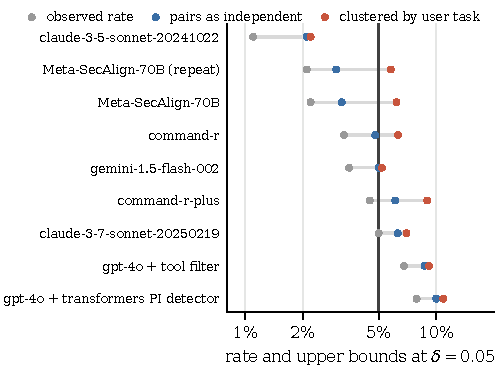
\includegraphics[width=\columnwidth]{fig_agentdojo.pdf}
\caption{The nine AgentDojo pipelines with the lowest attack success rates: observed rate, the Clopper-Pearson bound
that treats task pairs as independent, and the cluster bootstrap-t bound by user task (injection tasks fixed). Only the
top pipeline certifies 5\% once clustered; gemini-1.5-flash-002's per-pair bound is 0.050, a pass. ``Repeat'' and
the suffixes are AgentDojo's prompt-injection defences. From 200,000 bootstrap draws.}
\label{fig:agentdojo}
\end{figure}

\section{A Certificate in Human Terms}
\label{sec:human}

Every certificate above is in a judge's terms. Against XSTest's published human labels \citep{rottger2024xstest}, the
guard behind our refusal numbers recalls 0.92 of full refusals on safe prompts, but its false-alarm rate against full
refusal runs from 0.03 to 0.44 across the five released models, following each model's share of partial refusals;
against full or partial refusal it is 0.01 to 0.19, which is Section~\ref{sec:carry} on other people's models: its error rates
belong to a model. One annotator, an author, labelled 220 responses, 109 of the pre-update model and 111 of the updated policy, on a
stratified sheet read with its design weights; the sheet hid which policy wrote each response and shuffled the order. In strict refusals the two policies are level (10.7\% and 10.6\%).
From these labels, at $\delta=0.05$, a stratum-wise Clopper-Pearson construction certifies that the updated policy
refuses outright at most 20.1\% of its responses to the pool of 490 benign prompts; the \SWT{} gives 13.9\%, without a
guarantee. The policy is the update's last checkpoint (step 200), not the one its gate returned (step 175). The constraint the update was trained under, a refusal rate at most 2 points above the pre-update model's,
is certified by nothing in these labels: the limit on the difference is $+16.5$ points exact and $+6.4$ approximate. We
fixed these limits after the sheet's rates were known, so this is a computation, not a registered test.

The relative certificate is a question of budget (Appendix~\ref{app:human}). Pairing the two policies on the same prompts
cuts the labels needed about threefold; at a true difference near zero, about 420 labelled prompt pairs give an even
chance of certifying the 2-point margin with an approximate limit, and the exact limit is about twice as wide. The
samples (from the returned checkpoint, step 175, while the budget uses step 200's rates), guard scores and analysis for 300
pairs are prepared; the labels have not been collected.

\section{What This Means for a Release Gate}
\label{sec:gate}

For a regression gate on an updated policy, the measurements above suggest the following practice.
\begin{itemize}
\item \textbf{Label the updated policy's own responses at every update.} A rubric judge's error rates, measured on
  the previous version, did not carry across an update that targeted the judged label, in any of three seeds; a second
  judge's did, so a carry cannot be assumed (Section~\ref{sec:carry}). A judge can still reduce variance when its gold
  labels come from the updated policy.
\item \textbf{Use an exact bound at rare rates.} With no positive observed at $\delta=0.05$, 299 labels certify 1\%, 149
  certify 2\% and 59 certify 5\%. The designs we tried gained at most 1.2 there, and only under approximate limits.
\item \textbf{Do not use a plain Student-t or normal limit on a small rate,} nor a judge-assisted estimator's normal
  limit. Where a judge assists, use its logit with a bootstrap-t limit, only with 10 or more gold labels in each class (a
  threshold settled on these results and not confirmed), and report how often the limit declines.
\item \textbf{State what is sampled.} On a benchmark that crosses tasks with attacks, cluster by what the certificate
  treats as sampled, and say which factor is held fixed.
\item \textbf{Pair the two versions for a relative constraint.} Labelling both on the same prompts cuts the budget about
  threefold, by our design calculation.
\item \textbf{Treat a sequence of updates as a sequence of tests.} We studied one update at a time. A safety set whose
  result informed the next candidate is no longer independent of it, and $k$ gates at level
  $\delta$ each bound the chance of any wrong release only by $k\delta$; fresh safety sets and a split of $\delta$ across
  versions keep the guarantee, at a cost in labels that we did not measure.
\item \textbf{Stratify on the previous version only at rates from about 5\% to 80\% and for a costly label}, with the \SWT{}, and expect
  little if the update reorders prompts.
\item \textbf{Report how often the gate declines.} A gate that never passes is valid; how often it declines is its
  cost.
\end{itemize}

\section{Related Work}

\textbf{Seldonian algorithms and high-confidence improvement} \citep{thomas2015hcope,thomas2015hcpi,thomas2019preventing,metevier2019,giguere2022}
supply the gate we study; Safe RLHF \citep{dai2024saferlhf} trains against a learned cost with a Lagrange multiplier and
has no held-out test of what it returns. \textbf{Certificates of LLM behaviour} \citep{chaudhary2024knowledge,chaudhary2025bias}
use Clopper-Pearson bounds over a prompt distribution, the bias certificate in a detector's terms; we measure when such
bounds hold under stratified, judge-assisted and clustered sampling. \textbf{Error bars for evaluations}:
\citet{miller2024errorbars} sets out standard errors for evaluations, including clustered ones, and
\citet{bowyer2025clt} show the failure of normal intervals at small $n$; we add the one-sided, selection-robust setting and crossed designs,
for which multiway variances \citep{cameron2011multiway} and two-way bootstraps \citep{owen2007pigeonhole,menzel2021bootstrap}
exist. \textbf{Risk control} \citep{bates2021rcps,angelopoulos2024crc,angelopoulos2025ltt,zollo2024prc} calibrates a
wrapper around a fixed model; we certify a policy that training changed, on a label a judge defines.
\textbf{Prediction-powered inference} \citep{angelopoulos2023ppi,angelopoulos2023ppipp,fisch2024stratppi,zrnic2024ppboot,boyeau2025autoeval,zrnic2024active,gligoric2025cdi}
is the family whose finite-sample behaviour Section~\ref{sec:valid} measures. \textbf{Judge bias and label shift}
\citep{zheng2023judge,souly2024strongreject,saerens2002,lipton2018} motivate the carried bound, whose assumption of fixed
error rates Section~\ref{sec:carry} tests across an update. \textbf{Rare behaviours} below the rates we certify are
estimated, not certified, by \citet{wu2025rare} and \citet{jones2025forecasting}.

\section{Limitations}

Outside Section~\ref{sec:human} and XSTest's published labels, every refusal label is a guard model's, and our own human
labels are one annotator's, with no agreement statistic. Our trained policies are 1.5B and 2B parameters on one consumer GPU;
the frontier evidence is certificates on published traces. The new prompts come from one benchmark, and the policy that
reordered the prompts is one run of one model on one label; the three seeds of the targeted run share prompts, threshold
and gold label. The strata rule was chosen on the pools that first measured it and confirmed afterwards, and the
confirmation kept six of its eight predictions; the \SWT{} became our recommended limit after the first confirmation pool,
where the Wilson-type limit failed at 82\%. The approximate limits we recommend have no finite-sample guarantee, and
several hold partly by abstaining. The crossed-benchmark certificate takes the benchmark's injection tasks as given.

\section{Conclusion}

A rate with an error bar is not a release gate. The guarantee belongs to the whole procedure: how the update was chosen,
how the sample was drawn and what produced the label. Where we could check against a known truth, exact bounds held on
data sampled as they assume, and three shortcuts failed: a normal limit at small rates, a per-pair bound on a crossed
benchmark, and a judge's calibration carried to another population or, for a rubric judge in the one targeted set-up we ran
(three seeds), across an update that targeted the label.
Strata from the pre-update model help a little, at mid rates, under an approximate limit. For a regression gate on an
updated policy, the practical rule is to label the updated policy's own responses each time, bound them exactly where
the rate is small, and report how often the gate declines.

\bibliography{references}

\appendix

\section{Definitions}
\label{app:defs}

\paragraph{Labels alone.} For $s$ positives among $n$ 0/1 labels, Clopper-Pearson's upper limit is
$\mathrm{Beta}^{-1}(1-\delta;\,s+1,\,n-s)$, and $1-\delta^{1/n}$ at $s=0$. With no positive, the smallest sample that
certifies a threshold $\tau$ is $n\ge\ln\delta/\ln(1-\tau)$: 299 labels for 1\% at $\delta=0.05$, 149 for 2\%, 59 for
5\%. For labels in $[0,1]$ the exact choices are Hoeffding's \citep{hoeffding1963}, Bentkus's \citep{bentkus2004},
Anderson's \citep{learnedmiller2019} and the betting bound \citep{waudbysmith2024betting}. Wilson's bound
\citep{wilson1927} is the smallest $m>\hat p$ with $m-\hat p\ge z_{1-\delta}\sqrt{m(1-m)/n}$.

\paragraph{Stratified limits.} With strata $h$ of population share $W_h$, $n_h$ labels, $s_h$ positives and rates
$\hat p_h$, $\hat\mu=\sum_hW_h\hat p_h$. The \SWL{} is the smallest $m>\hat\mu$ with
$m-\hat\mu\ge z_{1-\delta}\sqrt{\sum_hW_h^2p_h(m)(1-p_h(m))/n_h}$, where $p_h(m)$ shifts every stratum's rate by
$m-\hat\mu$, clipped to $[0,1]$; it is a heuristic, not the inversion of a stratified score test. The \SWT{} is
$\hat\mu+t\sqrt{\sum_hW_h^2\tilde p_h(1-\tilde p_h)/(n_h-1)}$ with $\tilde p_h=(s_h+1/2)/(n_h+1)$ and a Student-t
quantile at Satterthwaite's degrees of freedom \citep{satterthwaite1946}. For a claim about the population a pool of $N$
prompts was drawn from, both add $\sum_hW_h(\hat p_h-\hat\mu)^2/N$ to the variance, the first-phase term of two-phase
sampling \citep{neyman1938,cochran1977}.

\paragraph{A judge.} With $n$ gold labels $e$, the judge's feature $f$ on them and on $N_u$ unlabelled responses, PPI++
\citep{angelopoulos2023ppipp} estimates $\hat p=\overline{e}+\gamma(\overline{f}_{\text{unl}}-\overline{f}_{\text{lab}})$ with
$\gamma=\mathrm{cov}(e,f)/((1+n/N_u)\mathrm{var}(f))$ and variance $V=\mathrm{var}(e-\gamma f)/n+\gamma^2\mathrm{var}_{\text{unl}}(f)/N_u$;
the published limit is $\hat p+z_{1-\delta}\sqrt V$. StratPPI \citep{fisch2024stratppi} applies the correction within
strata. PPBoot \citep{zrnic2024ppboot} uses a percentile of bootstrap estimates. The bootstrap-t limit
\citep{hall1988} resamples the labelled responses $B$ times (within strata where stratified), redraws each unlabelled
mean, and sets $U=\hat p-t^*_\delta\sqrt V$ with $t^*_\delta$ the $\delta$-quantile of $(\hat p^*_b-\hat p)/\sqrt{V^*_b}$.

\paragraph{Clustered data.} With clusters $c$ (user tasks) of sizes $n_c$ and successes $s_c$, $\hat p=\sum s_c/\sum
n_c$ and $se=\sqrt{C/(C-1)\sum_c(s_c-\hat pn_c)^2}/\sum_cn_c$; the limit is a bootstrap-t with whole clusters resampled.
For crossed clusters, the multiway variance is $V_u+V_{\text{inj}}-V_p$ \citep{cameron2011multiway}, and the pigeonhole
bootstrap \citep{owen2007pigeonhole} resamples both kinds of task independently.

\paragraph{Effective sample size.} $\mathrm{ESS}=(w_{\text{base}}/w_A)^2$ at equal labels and $\delta$. Unless stated,
$w$ is measured from the truth ($\mathrm{ESS}_{\text{truth}}$); the first strata study measures it from the estimate
($\mathrm{ESS}_{\text{est}}$). A design that removes a share $G$ of the variance has a predicted ESS of $1/(1-G)$; for
reference-rate strata $G\approx\mathrm{ICC}_{\text{cand}}\,\omega^2\,\mathrm{rel}(k)\,c_H$, with the updated policy's
intraclass correlation, the correlation $\omega$ of a prompt's pre- and post-update rates, the reliability
$\mathrm{rel}(k)=k\,\mathrm{ICC}_{\text{ref}}/(1+(k-1)\mathrm{ICC}_{\text{ref}})$ of a $k$-sample reference rate, and
$c_H=0.96$ at $H=8$. A judge with squared correlation $\rho^2$ to the gold label gives about $1/(1-\rho^2)$ when
unlabelled responses are plentiful.

\paragraph{The carried bound.} With recall $r$, false-alarm rate $f$ and flag rate $q=rp+f(1-p)$, $p=(q-f)/(r-f)$
\citep{rogan1978}; the carried bound combines one-sided limits on the three at $\delta/3$ each.

\section{The Full Validity Table}
\label{app:validity}

Tables~\ref{tab:fullA} to~\ref{tab:fullD} give every row. Rows in bold are bounds we do not use in that setting and
that are over their level there. Rows 1, 3 to 5 and 15 are exact computations over binomial counts on a harm pool from a
companion training run (Qwen2.5-0.5B policies; an unpublished paper) whose per-response labels were lost; its printed rate pins the count to
121 to 124 positives of 3,600, and every count in that range is computed exactly. Rows 37 to 55 were registered before they were run, and so were rows 14, 30 and 31, by a commit whose order
rests on its local time (Appendix~\ref{app:record}).

\begin{table*}[p]
\centering
\scriptsize
\setlength{\tabcolsep}{3pt}
\begin{tabular}{@{}r p{2.8cm} p{2.0cm} p{3.9cm} l p{2.1cm} p{2.0cm} p{1.9cm}@{}}
\toprule
\textbf{\#} & \textbf{bound} & \textbf{kind} & \textbf{setting} & \textbf{$\delta$} & \textbf{miss, per cell} & \textbf{cells over / unresolved / at or under} & \textbf{largest 95\% upper limit of a cell's miss (cells over after correction)} \\
\midrule
1 & Clopper-Pearson & exact (binary labels) & real harm labels, trained-policy pool, 121--124 positives of 3,600, n 200--2,400 & 0.10 & 0.066--0.096 & 0 / 0 / 20 & 0.096 (0) \\
2 & Clopper-Pearson & exact & the judge plasmodes (App.~\ref{app:judge}), every cell & 0.05 & 0--0.052 & 0 / 2 / 40 & 0.059 (0) \\
3 & betting mixture & exact (bounded) & same pool as row 1 & 0.10 & 0.007--0.018 & 0 / 0 / 20 & 0.018 (0) \\
4 & Bentkus & exact (bounded) & same pool & 0.10 & 0.017--0.037 & 0 / 0 / 20 & 0.037 (0) \\
5 & Hoeffding, Anderson & exact (bounded) & same pool & 0.10 & 0.000 & 0 / 0 / 40 & 0.000 (0) \\
6 & stratified Wilson-type limit & approximate & 4 mid-rate labels (9--95\%), real Granite-3.3-2B responses, $n_s$ 100--200, 3 checkpoints & 0.05 / 0.10 & 0.017--0.054 / 0.058--0.097 & 0 / 3 / 21; 0 / 0 / 24 & 0.061 (0); 0.106 (0) \\
7 & the Wilson-type limit & approximate & label pushed by the Lagrangian, $n_s$ 200 & 0.05 / 0.10 & 0.011--0.023 / 0.040--0.064 & 0 / 0 / 2; 0 / 0 / 2 & 0.027 (0); 0.071 (0) \\
8 & the Wilson-type limit on a design-weighted sheet & approximate & sheets re-drawn by their real sampling rule & 0.05 & 0--0.060 & 1 / 1 / 16 & 0.067 (0) \\
9 & PPI++ with a bootstrap-t limit & approximate & the judge plasmodes (App.~\ref{app:judge}), every cell and feature & 0.05 & 0--0.054 & 0 / 13 / 155 & 0.061 (0) \\
10 & cluster bootstrap-t, by user task & approximate & AgentDojo, 28 pipelines, scheme (a) & 0.05 & 0.013--0.051 & 0 / 2 / 26 & 0.058 (0) \\
11 & StratPPI estimator with a bootstrap-t limit, proportional allocation & approximate & reference-rate strata, 5 mid-rate labels, $n_s$ 100--200; judge-logit strata, n 100--1,000 & 0.05 & 0.024--0.045; 0.001--0.056 & 0 / 0 / 28; 0 / 5 / 23 & 0.051 (0); 0.064 (0) \\
12 & the same estimator and limit, redrawn with replacement & approximate & reference-rate strata, 5 mid-rate labels, $n_s$ 100--200 & 0.05 / 0.10 & 0.030--0.050 / 0.069--0.100 & 0 / 0 / 28; 0 / 1 / 27 & 0.052 (0); 0.103 (0) \\
13 & Clopper-Pearson, random draws with replacement (the control) & exact & the same 5 labels and sizes & 0.05 / 0.10 & 0.029--0.050 / 0.050--0.097 & 0 / 0 / 28; 0 / 0 / 28 & 0.052 (0); 0.100 (0) \\
14 & pigeonhole bootstrap-t & approximate & AgentDojo, 28 pipelines, schemes (a); (b); (c) & 0.05 & at most 0.004; 0.037; 0.042 & 0 / 0 / 28; 0 / 0 / 28; 0 / 0 / 28 & 0.007 (0); 0.043 (0); 0.048 (0) \\
15 & \textbf{Student-t} & fails at low rates & same pool as row 1, n 200--2,400 & 0.10 & \textbf{0.104--0.195} & 20 / 0 / 0 & 0.195 (20) \\
16 & \textbf{the Wilson-type limit and the pooled Wilson bound at rare rates} & in the stored design, not over at $\delta$ 0.05; over in 2 cells at 0.10 & harm labels at 1--2\%, $n_s$ 100--200, 3 checkpoints & 0.05 / 0.10 & 0--0.048 / \textbf{0--0.126} & 0 / 0 / 24; 2 / 1 / 21 & 0.054 (0); 0.136 (2) \\
17 & \textbf{the Wilson-type limit, redrawn with replacement} & over on the two labels at rates of 65\% and above & reference-rate strata, 5 mid-rate labels, $n_s$ 100--200 & 0.05 / 0.10 & \textbf{0.017--0.062 / 0.056--0.113} & 7 / 1 / 20; 6 / 2 / 20 & 0.065 (7); 0.116 (4) \\
18 & \textbf{pooled Wilson bound, random draws with replacement} & over in 6 and 10 of the 28 cells & the same 5 labels and sizes & 0.05 / 0.10 & \textbf{0.031--0.069 / 0.069--0.128} & 6 / 0 / 22; 10 / 3 / 15 & 0.071 (6); 0.131 (10) \\
\bottomrule
\end{tabular}

\caption{Miss rate against $\delta$, rows 1 to 18. Cells are counted as over / unresolved / at or under $\delta$; the next
column is the largest upper end of a 95\% interval for a cell's miss rate, with the cells still over after a
Bonferroni correction in brackets (for the exact binomial rows, the largest exact miss and the cells above $\delta$). Draws per cell: 4,000 to 40,000. AgentDojo schemes: (a) user tasks resampled, injection tasks fixed; (b) the reverse;
(c) both. ``Redrawn with replacement'' draws each stratum's prompts with replacement, the limit of a pool far larger
than the safety set.}
\label{tab:fullA}
\end{table*}

\begin{table*}[p]
\centering
\scriptsize
\setlength{\tabcolsep}{3pt}
\begin{tabular}{@{}r p{2.8cm} p{2.0cm} p{3.9cm} l p{2.1cm} p{2.0cm} p{1.9cm}@{}}
\toprule
\textbf{\#} & \textbf{bound} & \textbf{kind} & \textbf{setting} & \textbf{$\delta$} & \textbf{miss, per cell} & \textbf{cells over / unresolved / at or under} & \textbf{largest 95\% upper limit of a cell's miss (cells over after correction)} \\
\midrule
19 & \textbf{PPI++ with a normal limit} & fails in most cells & the judge plasmodes (App.~\ref{app:judge}) & 0.05 & \textbf{0.041--0.241} & 126 / 29 / 13 & 0.255 (87) \\
20 & \textbf{StratPPI's normal limit, proportional allocation} & fails at these sizes & reference-rate strata; judge-logit strata & 0.05 & \textbf{0.024--0.086; 0.054--0.239} & 9 / 5 / 14; 26 / 2 / 0 & 0.094 (7); 0.252 (25) \\
21 & \textbf{StratPPI's normal limit, the paper's allocations (oracle; heuristic)} & fails & reference-rate strata; judge-logit strata & 0.05 & \textbf{up to 0.110; 0.217; up to 0.219; 0.90} & 9 / 3 / 14; 11 / 0 / 15; 28 / 0 / 0; 24 / 1 / 3 & 0.119 (8); 0.229 (11); 0.232 (25); 0.912 (24) \\
22 & \textbf{StratPPI estimator with a bootstrap-t limit, oracle or heuristic allocation} & fails & the same cells & 0.05 & \textbf{up to 0.078; 0.174; up to 0.083; 0.90} & 6 / 3 / 17; 11 / 1 / 14; 14 / 11 / 3; 14 / 0 / 14 & 0.086 (5); 0.185 (11); 0.092 (9); 0.910 (14) \\
23 & \textbf{PPBoot, percentile limit (basic; power-tuned)} & fails at these sizes & judge-logit cells, unstratified & 0.05 & \textbf{up to 0.133; 0.148} & 7 / 6 / 1; 12 / 2 / 0 & 0.144 (5); 0.160 (11) \\
24 & \textbf{Clopper-Pearson over pairs} & fails on a crossed design & AgentDojo, 28 pipelines, schemes (a); (b); (c) & 0.05 & \textbf{0.042--0.268; 0.060--0.340; 0.195--0.350} & 27 / 0 / 1; 28 / 0 / 0; 28 / 0 / 0 & 0.282 (26); 0.355 (27); 0.365 (28) \\
25 & \textbf{cluster bootstrap-t by user task, when injection tasks are sampled} & fails & AgentDojo, schemes (b); (c) & 0.05 & \textbf{up to 0.258; 0.275} & 21 / 0 / 7; 24 / 0 / 4 & 0.272 (20); 0.289 (24) \\
26 & \textbf{larger of the two clustered bounds} & holds under (a) only & AgentDojo, schemes (a); (b); (c) & 0.05 & at most 0.029; \textbf{up to 0.066; 0.089} & 0 / 0 / 28; 4 / 0 / 24; 16 / 3 / 9 & 0.034 (0); 0.074 (3); 0.098 (15) \\
27 & \textbf{pigeonhole bootstrap, basic limit} & fails & AgentDojo, schemes (a); (b); (c) & 0.05 & \textbf{up to 0.174; 0.178; 0.278} & 5 / 0 / 23; 14 / 1 / 13; 27 / 0 / 1 & 0.187 (5); 0.190 (10); 0.292 (26) \\
28 & \textbf{PPI on a stratified sheet read as an i.i.d. sample} & fails & three judge wordings, labels planted at three rates & 0.05 & \textbf{0--0.989} & 7 / 0 / 11 & 0.992 (7) \\
29 & \textbf{the judge's rate alone} & fails & the judge plasmodes (App.~\ref{app:judge}) & 0.05 & \textbf{0--1.000} & 30 / 0 / 12 & 1.000 (30) \\
30 & \textbf{multiway cluster variance with a t quantile} & fails & AgentDojo, schemes (a); (b); (c) & 0.05 & \textbf{up to 0.136; 0.175; 0.179} & 5 / 0 / 23; 8 / 3 / 17; 26 / 1 / 1 & 0.147 (5); 0.187 (7); 0.191 (25) \\
31 & \textbf{two clustered margins added in quadrature} & over in one cell under (c) & AgentDojo, schemes (a); (b); (c) & 0.05 & at most 0.015; 0.046; \textbf{0.058} & 0 / 0 / 28; 0 / 0 / 28; 1 / 1 / 26 & 0.020 (0); 0.053 (0); 0.066 (0) \\
\bottomrule
\end{tabular}

\caption{Miss rate against $\delta$, rows 19 to 31. Cells are counted as over / unresolved / at or under $\delta$; the next
column is the largest upper end of a 95\% interval for a cell's miss rate, with the cells still over after a
Bonferroni correction in brackets (for the exact binomial rows, the largest exact miss and the cells above $\delta$).}
\label{tab:fullB}
\end{table*}

\begin{table*}[p]
\centering
\scriptsize
\setlength{\tabcolsep}{3pt}
\begin{tabular}{@{}r p{2.8cm} p{2.0cm} p{3.9cm} l p{2.1cm} p{2.0cm} p{1.9cm}@{}}
\toprule
\textbf{\#} & \textbf{bound} & \textbf{kind} & \textbf{setting} & \textbf{$\delta$} & \textbf{miss, per cell} & \textbf{cells over / unresolved / at or under} & \textbf{largest 95\% upper limit of a cell's miss (cells over after correction)} \\
\midrule
32 & stratified Wald-t limit, 8 reference-rate strata & approximate & 5 mid-rate labels, real Granite-3.3-2B responses, $n_s$ 100--200, the draws of the StratPPI row & 0.05 / 0.10 & 0.007--0.036 / 0.027--0.080 & 0 / 0 / 28; 0 / 0 / 28 & 0.042 (0); 0.088 (0) \\
33 & the same limit, redrawn with replacement & approximate & the same 5 labels and sizes & 0.05 / 0.10 & 0.007--0.038 / 0.026--0.086 & 0 / 0 / 28; 0 / 0 / 28 & 0.040 (0); 0.088 (0) \\
34 & the same limit with the term for a sampled pool & approximate & a claim about the prompt source: the pool redrawn and the strata rebuilt, the same 5 labels and sizes & 0.05 / 0.10 & 0.007--0.050 / 0.031--0.095 & 0 / 1 / 27; 0 / 0 / 28 & 0.055 (0); 0.101 (0) \\
35 & \textbf{stratified Wald-t limit on a synthetic i.i.d. grid} & over in 5 of 18 cells at each $\delta$ & six strata profiles, $n_s$ 100--400, binomial strata & 0.05 / 0.10 & \textbf{0--0.111 / 0.086--0.147} & 5 / 5 / 8; 5 / 5 / 8 & 0.121 (4); 0.158 (4) \\
36 & \textbf{the Wilson-type limit on the same grid} & over in 1 and 4 of 18 cells & the same profiles and sizes & 0.05 / 0.10 & \textbf{0--0.057 / 0.086--0.135} & 1 / 2 / 15; 4 / 5 / 9 & 0.065 (0); 0.146 (2) \\
37 & stratified Wald-t limit inside the training loop, 8 strata & approximate & synthetic bandit, Lagrangian GRPO, 4 environments, the pool's own rate, 8,000 runs a cell & 0.05 / 0.10 & 0.029--0.052 / 0.072--0.100 & 0 / 1 / 3; 0 / 1 / 3 & 0.057 (0); 0.107 (0) \\
38 & the same limit with the sampled-pool term & over in 1 of 4 cells at each $\delta$ & the same runs, the population's rate & 0.05 / 0.10 & 0.047--0.057 / 0.093--0.107 & 1 / 1 / 2; 1 / 0 / 3 & 0.062 (1); 0.114 (0) \\
39 & stratified Wald-t limit, a costly label stratified on a cheap reference rate & over in 1 and 2 of 32 cells & XSTest human labels of five released models, 8 mid-rate labels, two stratifiers, $n_s$ 50--100, redrawn with replacement & 0.05 / 0.10 & 0--0.053 / 0.021--0.108 & 1 / 0 / 31; 2 / 0 / 30 & 0.055 (0); 0.111 (2) \\
40 & betting mixture on user-task rates; on the pair rate & exact (bounded) & AgentDojo, 28 pipelines, user tasks redrawn across the table (a) and within suites (a\_s); truth: the average over user tasks; the pair rate & 0.05 & at most 0.007; 0.005; 0.006; 0.003 & 0 / 0 / 28; 0 / 0 / 28; 0 / 0 / 28; 0 / 0 / 28 & 0.010 (0); 0.008 (0); 0.010 (0); 0.005 (0) \\
41 & cluster bootstrap-t, by user task, redrawn within suites & approximate & AgentDojo, 28 pipelines, scheme (a\_s) & 0.05 & 0.003--0.042 & 0 / 0 / 28 & 0.049 (0) \\
42 & \textbf{cluster bootstrap-t by user task, injection tasks redrawn within suites} & fails & AgentDojo, schemes (b\_s); (c\_s) & 0.05 & \textbf{up to 0.231; 0.249} & 11 / 1 / 16; 19 / 2 / 7 & 0.244 (11); 0.262 (18) \\
43 & two clustered margins in quadrature, redrawn within suites & approximate & AgentDojo, schemes (a\_s); (b\_s); (c\_s) & 0.05 & at most 0.016; 0.037; 0.040 & 0 / 0 / 28; 0 / 0 / 28; 0 / 0 / 28 & 0.020 (0); 0.044 (0); 0.046 (0) \\
\bottomrule
\end{tabular}

\caption{Miss rate against $\delta$, rows 32 to 43. Cells are counted as over / unresolved / at or under $\delta$; the next
column is the largest upper end of a 95\% interval for a cell's miss rate, with the cells still over after a
Bonferroni correction in brackets (for the exact binomial rows, the largest exact miss and the cells above $\delta$). Rows 32 to 36 are the \SWT{} and, on a
synthetic grid, it and the Wilson-type limit; 37 to 39 the same limit inside the training loop and on a costly human
label; 40 to 43 AgentDojo with an exact bound and with tasks redrawn within the benchmark's suites.}
\label{tab:fullC}
\end{table*}

\begin{table*}[p]
\centering
\scriptsize
\setlength{\tabcolsep}{3pt}
\begin{tabular}{@{}r p{2.8cm} p{2.0cm} p{3.9cm} l p{2.1cm} p{2.0cm} p{1.9cm}@{}}
\toprule
\textbf{\#} & \textbf{bound} & \textbf{kind} & \textbf{setting} & \textbf{$\delta$} & \textbf{miss, per cell} & \textbf{cells over / unresolved / at or under} & \textbf{largest 95\% upper limit of a cell's miss (cells over after correction)} \\
\midrule
44 & stratified Wald-t limit, a second model family, redrawn with replacement & approximate & Qwen2.5-1.5B-Instruct, refusal label (18--19\%), 8 reference-rate strata, steps 100 and 200, $n_s$ 100--200 & 0.05 / 0.10 & 0.033--0.046 / 0.077--0.092 & 0 / 0 / 4; 0 / 0 / 4 & 0.048 (0); 0.095 (0) \\
45 & the Wilson-type limit, the same & approximate & the same cells & 0.05 / 0.10 & 0.033--0.041 / 0.086--0.092 & 0 / 0 / 4; 0 / 0 / 4 & 0.043 (0); 0.095 (0) \\
46 & the stratified Wald-t limit with the term for a sampled pool, a second model family & over in 1 of 4 cells at $\delta$ 0.10 & a claim about the prompt source, the same label, steps and sizes & 0.05 / 0.10 & 0.036--0.051 / 0.085--0.111 & 0 / 1 / 3; 1 / 0 / 3 & 0.056 (0); 0.118 (1) \\
47 & stratified Clopper-Pearson: a stratified draw's pooled count plus the allocation's slack & exact (binary labels) & 116 cells: real responses (58), a costly label (40), a synthetic grid (18), drawn with replacement within strata, $n_s$ 50--400 & 0.05 / 0.10 & 0--0.048 / 0--0.093 & 0 / 0 / 116; 0 / 0 / 116 & 0.048 (0); 0.093 (0) \\
48 & stratified betting bound (union-intersection) & exact (bounded) & the same cells & 0.05 / 0.10 & 0--0.001 / 0--0.007 & 0 / 0 / 116; 0 / 0 / 116 & 0.002 (0); 0.010 (0) \\
49 & cluster bootstrap-t, by user task, against a fitted crossed model & approximate & AgentDojo, 28 pipelines, tables drawn from a fitted crossed model with injection tasks fixed (P\_a); truth: the model's rate & 0.05 & 0.001--0.044 & 0 / 0 / 28 & 0.051 (0) \\
50 & \textbf{the same, both kinds of task drawn from the model} & fails & the same, scheme (P\_c) & 0.05 & \textbf{up to 0.247} & 18 / 3 / 7 & 0.260 (17) \\
51 & betting mixture on user-task rates; on the pair rate, against a fitted crossed model & exact (bounded) & the same, scheme (P\_a); truth: the model's user-task average; its pair rate & 0.05 & at most 0.005; 0.003 & 0 / 0 / 28; 0 / 0 / 28 & 0.007 (0); 0.006 (0) \\
52 & pigeonhole bootstrap-t; two clustered margins in quadrature, against a fitted crossed model & approximate & the same, schemes (P\_a); (P\_c) for each & 0.05 & at most 0.011; 0.037; 0.016; 0.047 & 0 / 0 / 28; 0 / 0 / 28; 0 / 0 / 28; 0 / 0 / 28 & 0.014 (0); 0.043 (0); 0.021 (0); 0.054 (0) \\
53 & stratified Wald-t limit, a policy that training moved far, redrawn with replacement & approximate & Qwen2.5-1.5B-Instruct trained on the guard's refusal flag alone, refusal label (26\% at step 100, 58\% at step 200), the second family's pool and strata, $n_s$ 100--200 & 0.05 / 0.10 & 0.043--0.049 / 0.095--0.100 & 0 / 0 / 4; 0 / 0 / 4 & 0.051 (0); 0.103 (0) \\
54 & \textbf{the Wilson-type limit, the same} & over in all 4 cells at the 58\% rate & the same cells & 0.05 / 0.10 & \textbf{0.045--0.059 / 0.098--0.112} & 2 / 0 / 2; 2 / 1 / 1 & 0.062 (2); 0.115 (2) \\
55 & the stratified Wald-t limit with the term for a sampled pool, a policy that training moved far & approximate & a claim about the prompt source, the same label, steps and sizes & 0.05 / 0.10 & 0.040--0.048 / 0.085--0.094 & 0 / 0 / 4; 0 / 0 / 4 & 0.052 (0); 0.100 (0) \\
\bottomrule
\end{tabular}

\caption{Miss rate against $\delta$, rows 44 to 55. Cells are counted as over / unresolved / at or under $\delta$; the next
column is the largest upper end of a 95\% interval for a cell's miss rate, with the cells still over after a
Bonferroni correction in brackets (for the exact binomial rows, the largest exact miss and the cells above $\delta$). Rows 44 to 46 are the second model family after an update that kept its order of prompts, and 53 to 55 the same
family after a separate update, trained on the guard's flag alone, that reordered them; 47 and 48 exact stratified bounds; 49 to 52 AgentDojo against a fitted crossed model (schemes $P_a$, injection
tasks fixed, and $P_c$, both drawn), where only a bound that fails to compute counts as a miss.}
\label{tab:fullD}
\end{table*}

\paragraph{Abstention.} A bound that returns no limit, or a limit of 1, gives no certificate and cannot miss. The
bootstrap-t StratPPI limit returns none in up to 6\% of draws on the reference-rate strata (up to 8.6\% redrawn with
replacement) and in up to 52\% on the judge-logit strata at a 1.3\% rate; PPI++ with a bootstrap-t limit in up to 55\% of
draws where a sample of 225 holds about three positives; the clustered AgentDojo limits in up to 82\% of tables (the pigeonhole
bootstrap-t; the cluster bootstrap-t by user task in up to 15\% on these draws), for the pipelines with the fewest
successes. Counted as misses, the rows that hold would be over in up to 7 of 28 cells (row 12
at $\delta=0.05$), in 10 of 168 for row 9 and for 2 to 7 of 28 pipelines in the AgentDojo rows. Counted this way even an
exact bound can exceed its level: Clopper-Pearson returns 1 when every label is a positive, which at a 95\% label with a
safety set of 100 happens in 0.9\% of draws and takes it to 0.052 at $\delta=0.05$. The count measures how much of a
record is abstention, not validity.

\paragraph{The Wilson limit, exactly.} For an i.i.d.\ sample the Wilson limit's miss probability, computed by
enumeration, jumps just above each value the limit can take and falls until the next; averaged over rates it is under
$\delta$ below one half and over it above. At $n=100$ and $\delta=0.05$ it averages 0.042 over rates of 5--20\% and 0.056
over 80--95\%. Redrawn with replacement, the \SWL{} is over its level in 7 of 28 mid-rate cells at $\delta=0.05$, all on
the two labels at rates of 65\% and above, and in none of the 16 at rates of 9--18\%; the pooled Wilson bound is over in
6 of 28. Rare labels take Clopper-Pearson or a betting bound.

\section{Selection and the Training Loop}
\label{app:pipeline}

The resampling studies hold the candidate fixed. Two checks test the gate with selection in it. With the training code of
our language-model runs (GRPO with a Lagrangian on the judged rate, a predicted safety test choosing the checkpoint)
applied to a synthetic bandit at four levels of between-prompt heterogeneity, 8 strata and 8,000 runs a cell, the \SWT{}
for the pool's own rate was over its level in none of its 8 cells (2 unresolved; largest miss 0.052 at $\delta=0.05$
and 0.100 at 0.10). With the sampled-pool term, for the population's rate, it was over in the least heterogeneous
environment at both deltas (0.057 and 0.107) and in no other cell; the Wilson-type limit with the term and the pooled
bound on a random split were over in none. With 4 strata and 500 runs a cell, the \SWT{} was over in one of four cells
(0.132 at $\delta=0.1$). In a classifier setting with a constraint on a difference of true-positive rates,
rerandomised and stratified candidate/safety splits, across eleven split rules, 2,000 seeds per arm and candidates built
to overfit the balancing statistics, returned a passing, truly violating candidate in at most 1 of 2,000 runs under
Clopper-Pearson; a tight Wald test on the same runs, sensitive enough to show a leak, fell below the truth in at most
0.055 of runs at $\delta=0.05$.

\section{Strata from the Pre-Update Model in Detail}
\label{app:strata}

\paragraph{First pools.} With $k=8$ and $H=8$ on Granite-3.3-2B's responses, $\mathrm{ESS}_{\text{est}}$ at $\delta=0.10$
was 2.4 for over-refusal (rate 17\%, $\mathrm{ICC}_{\text{ref}}$ 0.72), 5.1--5.3 for refusal of plainly harmful requests
(66\%, 0.86) and 1.4 for non-refusal of encoded requests (9\%, 0.50); placebo strata cut on a permuted reference rate gave
1.00 to 1.04 with 4 strata on every label but the one at 93\%. When the Lagrangian pushed the stratified label itself,
the gain was 2.1--2.2, with no compression of the between-prompt spread and the order of prompts kept ($\omega$ 0.92),
in a run whose rate ended within 0.4 to 3.4 points of the reference's. The rule registered in advance collapsed to one to
three strata, because most prompts have an 8-sample reference rate of exactly 0 or 1; equal rank strata with random ties
were adopted on the same pools, and the truth used for coverage, which carried a fixed offset shared by every draw,
became the mean of the half of the responses the draws come from; these gains were thus measured on the data that chose
the rule (Appendix~\ref{app:record}).

\paragraph{The pre-flight} ranks the gain (Spearman 0.84 between predicted and realised $\mathrm{ESS}_{\text{est}}$ over
432 cells at $\delta=0.10$) and over-predicts its size. On new prompts it was within 20\% at all three mid rates with the
updated policy's two quantities measured on responses the draws do not use; from the reference samples alone it
predicted 2.58, 4.12 and 2.22, and the realised gains were 27\% to 41\% lower.

\paragraph{Against StratPPI.} On the same strata and draws, StratPPI as published is shorter partly because its normal
limit runs over its level (Table~\ref{tab:stratppi}); with a bootstrap-t limit and proportional allocation its estimator
holds, with a median ESS of 2.10 against 2.16 for the Wilson-type limit. At a safety set of 100 with 8 strata the
within-stratum regression on the reference rate adds nothing once the limit is valid; at 200, or with 4 strata, it adds
0.4 to 0.8. For a claim about the prompt source, with the pool redrawn and the strata rebuilt, limits without the
sampled-pool term fail: the Wilson-type limit is over in 17 of 28 cells and the bootstrap-t StratPPI limit in 21.

\begin{table*}[t]
\centering
\scriptsize
\setlength{\tabcolsep}{3pt}
\begin{tabular}{@{}p{4.2cm} r p{2.4cm} p{2.6cm} p{3.4cm}@{}}
\toprule
\textbf{label (rate)} & \textbf{$n_s$} & \textbf{the Wilson-type limit} & \textbf{StratPPI as published} & \textbf{StratPPI estimator, bootstrap-t limit} \\
\midrule
over-refusal (0.16) & 100 & 0.023; 2.39 & \textbf{0.066}; 4.11 & 0.042; 2.58 \\
over-refusal (0.16) & 200 & 0.024; 2.30 & 0.052; 3.46 & 0.042; 3.10 \\
over-refusal, pushed by the Lagrangian (0.18) & 100 & 0.024; 2.19 & 0.0558; 3.24 & 0.036; 2.43 \\
over-refusal, pushed (0.18) & 200 & 0.023; 2.13 & 0.045; 2.85 & 0.037; 2.49 \\
non-refusal, encoded prompts (0.09) & 100 & 0.034; 1.38 & \textbf{0.086}; 2.59 & 0.045; 1.43 \\
non-refusal, encoded prompts (0.09) & 200 & 0.027; 1.36 & \textbf{0.063}; 2.11 & 0.041; 1.59 \\
refusal, harmful prompts (0.65) & 100 & 0.047; 4.74 & \textbf{0.0564}; 6.30 & 0.033; 1.77 \\
refusal, harmful prompts (0.65) & 200 & 0.040; 5.19 & 0.045; 6.29 & 0.034; 5.35 \\
refusal, encoded prompts (0.93) & 100 & 0.054; 0.96 & 0.032; 0.78 & 0.031; 0.83 \\
refusal, encoded prompts (0.93) & 200 & 0.045; 1.12 & 0.026; 0.92 & 0.033; 1.03 \\
\bottomrule
\end{tabular}

\caption{Reference-rate strata at $\delta=0.05$: largest miss over checkpoints; ESS against a random split with a
pooled Wilson bound. Bold: more than two Monte Carlo standard errors over $\delta$ (above 0.0562 at 5,000 draws a cell;
the two cells nearest it carry a fourth digit).}
\label{tab:stratppi}
\end{table*}

\paragraph{The registered confirmation.} On three new pools (refusal rates 12\%, 82\%, 98\%), six of eight predictions
were kept. With a large pool the Wilson-type limit was over its level in none of 4 cells at 12\% and in all 4 at 82\%;
the bootstrap-t StratPPI limit was over in 1 of 8 mid-rate cells (0.105 at $\delta=0.10$, at 82\%) and in one at 98\%
(0.0524 at $\delta=0.05$); the \SWT{} in none of 8. For the source, the Wilson-type limit with the term was over at 82\%
with a safety set of 100 (0.058), where the \SWT{} with the term was over in none of 8. On the mixed pool at 46\%, nine of
ten predictions were kept and one could not be tested; it is weaker evidence, because its rate was aimed at and its
predictions were written after a dry run on a re-mix of the first pools' responses, and the reference rate largely
sorts its two sources into different strata. The second family's update, meant to reorder prompts, did not
(correlation 0.84; three of six predictions kept). A separate update of the same model, trained on the guard's flag
alone, did reorder them
(0.46): the \SWT{} stayed valid and gained 0.97 and 1.08, the Wilson-type limit was over in all 4 cells at 58\%, and four of
five predictions were kept; the one refuted is the check of the push's direction (refusal rose on the categories it was
meant to lower). By its registration, a failed direction check meant the policy had not moved; the rate nearly tripled
and the order of prompts moved further than in any other run, so we report it as moved, against that reading.

\paragraph{A costly label.} With XSTest's human labels on five released models' completions for its 250 safe prompts,
strata from the guard's rate over 8 Granite-3.3-2B reference responses, safety set 100 drawn with replacement, the
\SWT{}'s gain over eight mid-rate labels was 0.97 to 1.34 (median 1.18); it was over its level in 3 of 64 cells by at most
0.008. The Wilson-type limit gained 1.10 to 1.36 but was over in 8 of 32 cells at $\delta=0.05$.

\paragraph{Exact stratified bounds and the chance of certifying.} Over 116 cells drawn with replacement within strata,
Clopper-Pearson on the stratified draw's pooled count plus the allocation's slack, and a stratified betting bound
\citep{spertus2022sweeter}, kept their level everywhere. At a threshold where Clopper-Pearson on a random draw passes with
probability 0.8, the stratified Clopper-Pearson bound's power ESS on the 36 real-response cells at rates of 5\% to 95\%
was 1.11 (median; 0.27 to 1.83) and on the 32 costly-label cells 0.88; the betting bound's was 0.05; the \SWT{}'s 1.88.

\paragraph{The rule in one place.} For 8 equal rank strata of an 8-sample reference rate: a label that may be rare (under
about 5\%) or near one (above about 95\%) takes no strata and Clopper-Pearson or a betting bound; a mid-rate label (about 5\%
to 80\%) takes the \SWT{}, with the sampled-pool term for a claim about the prompt source; from about 80\% to 95\% a random
draw serves as well; where a finite-sample guarantee is required, Clopper-Pearson on a random draw; where the update may
reorder the prompts, the same limits, expecting little gain.

\section{Judges in Detail}
\label{app:judge}

\begin{table}[t]
\centering
\small
\begin{tabular}{@{}p{3.4cm}p{3.6cm}@{}}
\toprule
data & route \\
\midrule
a property code can verify & compute it on every response; Clopper-Pearson (exact) \\
gold labels, fewer than 10 in the rarer class & Clopper-Pearson on the labels; judge unused (exact) \\
gold labels, 10 or more in each class & PPI++ on the judge's logit, bootstrap-t limit (approximate) \\
gold labels from a stratified sheet & design-weighted labels, \SWL{} (approximate) \\
a calibration measured on another population & refused \\
\bottomrule
\end{tabular}
\caption{The routing rule, fixed before a constraint's labels are read. It was settled on the resampling results (20
cells) and has had no confirmation run. On the one stratified sheet design tested the
Wilson-type limit was over its level in 1 of 18 cells (0.060), and it can be over once the pool is large
(Section~\ref{sec:valid}); the \SWT{} is the safer choice
there, and an exact stratum-wise Clopper-Pearson construction (Section~\ref{sec:human}) where a guarantee is required.}
\label{tab:routing}
\end{table}

\paragraph{What a judge is worth.} For the compiled refusal judge against the guard's label (225 labels, 2,000 judged
draws), ESS against Clopper-Pearson on the labels is 1.11 for the 0/1 verdict, 1.15 for the probability, 1.61 for the
logit and 1.86 for a cross-fitted Platt score \citep{platt1999}. The logit carries more than the verdict.

\paragraph{Labels drawn within strata of the judge.} With labels allocated in proportion to stratum size, StratPPI's
estimator with a bootstrap-t limit was over its level in none of 28 cells (5 unresolved, largest miss 0.056; 5 would be
over if its returns of no limit counted as misses, 4 of them at the 1.3\% rate), with a median ESS of 2.54 at a 20\% rate
and 1.87 at 5\% with 10 strata, against 1.67 and 1.39 for unstratified PPI++ with the same limit. The 0.90 cell of
Table~\ref{tab:valid} is the rubric judge at a 5\% rate, 1,000 labels, 5 strata and the heuristic allocation: four
strata with judge probability under 0.001 hold 19\% of the positives at rates of 1.0--1.5\%, and their eight labels show
no positive in 91\% of draws.

\paragraph{The carried calibration, by seed.} Across the targeted update, recall differed in 2, 2 and 1 of six
wordings and the carried bound was over its level for 3, 3 and 2 (seed 0: misses 0.08, 0.23 and 0.80; the largest in
seeds 1 and 2 are 0.399 and 0.625); at step 100 it was over for 1, 1 and 4. Seeds 1 and 2 returned \NSF{} at their gate
(upper bounds 0.2317 and 0.2064 against a threshold of 0.2058; seed 0's step 175 had 0.1979 and was returned), so the
step-200 checkpoints analysed are not policies the gate returned; the question is what a carried calibration says about
an updated policy, which does not depend on that. We wrote down beforehand, in a note with no independent timestamp, that
a failure at step 200 would mean the earlier success was luck and no calibration carries across training; reading the
side-effect run as a control came after the result. WildGuard, as judge with the guard as gold, had false alarms of 1.0\%
before and 1.0\% to 1.7\% after; against the annotator's strict refusals after the update, WildGuard and the guard agree
equally well (design-weighted accuracy 0.930 and 0.929), and the compiled judge flags none of 18. WildGuard's own
calibration did not carry from the harmful pool to the benign one (85\% misses).

\paragraph{The mechanism we suspect.} By the guard and a surface pattern (a refusal opener and more than 40 words), on
the 500-response sets that both judges scored, 29 of the pre-update model's 100 guard flags are long refusals, against
83 of 93, 83 of 108 and 85 of 97 after the update in seeds 0, 1 and 2. Of the 93 guard-flagged refusals of seed 0 after
the update, the rubric judge called 90 answers. Of 18
such responses, the annotator labelled 12 refusals and 6 answers. WildGuard flagged 95\% of the guard-flagged responses
with the pattern and 92\% of those without. The rubric judge flagged 10\% of the pre-update model's guard-flagged
responses with the pattern and 25\% of those without (canonical wording); after the update, about 14 of 251 with it, against 3
of 29 before (no detectable change), and about 2 of 47 without it, against 18 of 71 before, so training changed both how many responses
have the pattern and how the judge reads the plain ones. The pattern is not a label, and no experiment here isolates the cause; the
two runs also differ in reward and set-up.

\section{Benchmarks in Detail}
\label{app:bench}

\paragraph{AgentDojo.} The published runs hold 19,380 episodes. Table~\ref{tab:agentdojo} gives six pipelines. The
bound clustered by user task returns no limit when the $\delta$-quantile of its bootstrap is not finite: on the fresh
draws of a registered run, in 9\% of the tables of the pipeline that certifies and in 16\% for the two Meta-SecAlign-70B
pipelines. Redrawing injection tasks within the benchmark's suites, the bound is over for 11 of 28 pipelines. Against
a fitted crossed logit-normal model with independent task effects, the same bound is over for none with injection
tasks fixed and for 18 of 28 with both kinds of task drawn; the multiway limit for 13 and the pigeonhole bootstrap-t for
none. Under the model, the pipeline that certifies on its published table certifies in 99\% of tables with the injection
tasks fixed under the bound clustered by user task, and in 35\% under the betting bound on user-task rates. The
certificate's bound is sensitive to the bootstrap's size when a handful of clusters hold every success: for the
defended model, at 4,000 draws it ranged from 0.058 to 0.107 over 30 seeds.

\begin{table*}[t]
\centering
\scriptsize
\setlength{\tabcolsep}{3pt}
\begin{tabular}{@{}p{3.0cm} r r r r r l r p{1.6cm}@{}}
\toprule
\textbf{pipeline} & \textbf{pairs} & \textbf{rate} & \textbf{per-pair bound} & \textbf{clustered by user task} & \textbf{clustered by injection task} & \textbf{``at most 5\%''} & \textbf{exact, user-task average} & \textbf{both kinds of task sampled} \\
\midrule
claude-3-5-sonnet-20241022 & 629 & 0.011 & 0.021 & 0.022 & 0.035 & pass & 0.048 & no limit \\
Meta-SecAlign-70B & 949 & 0.022 & 0.032 & 0.062 & 0.035 & NSF & 0.092 & 0.091 \\
command-r & 629 & 0.033 & 0.048 & 0.063 & 0.054 & NSF & 0.071 & 0.078 \\
claude-3-7-sonnet-20250219 & 949 & 0.050 & 0.063 & 0.070 & 0.104 & NSF & 0.119 & 0.107 \\
gpt-4o + tool\_filter & 629 & 0.068 & 0.087 & 0.092 & 0.106 & NSF & 0.107 & 0.115 \\
gpt-4o-2024-05-13 & 629 & 0.477 & 0.511 & 0.537 & 0.588 & NSF & 0.593 & 0.604 \\
\bottomrule
\end{tabular}

\caption{Targeted attack success on AgentDojo's published runs, upper bounds at $\delta=0.05$. The certificate is the
bound clustered by user task with injection tasks taken as fixed; the verdict column is for it. The exact column is the
betting bound on the user tasks' success rates, which bounds their average; the last column is the pigeonhole
bootstrap-t, which also takes injection tasks as sampled. Bootstrap bounds from 200,000 draws.}
\label{tab:agentdojo}
\end{table*}

\paragraph{A robot benchmark.} RoboDojo-RC Tier 1 \citep{machcha2026robodojo} publishes 120 trials per model, 20 on each
of six tasks the report selected; the harness's overheat termination is the label. With the six tasks taken as fixed,
the pooled Clopper-Pearson limit is valid for their mean \citep{hoeffding1956successes}. Table~\ref{tab:robot} shows what
120 trials resolve: a 2.5\% rate when nothing is observed, and not 5\% after two events; a 1\% claim with nothing
observed needs 299 trials. Taken as a sample of tasks, six tasks certify nothing useful. In an exploratory analysis, the
peak joint effort the rig reports predicts a stop (AUC 0.75 to 0.83 by model), partly mechanically, since the stop is an
overheat.

\begin{table}[t]
\centering
\scriptsize
\setlength{\tabcolsep}{2pt}
\resizebox{\columnwidth}{!}{\begin{tabular}{@{}l r r r r r p{2.6cm} r@{}}
\toprule
\textbf{model} & \textbf{n} & \textbf{stops} & \textbf{rate} & \textbf{upper, $\delta$ 0.05} & \textbf{upper, $\delta$ 0.10} & \textbf{``at most 5\%'' at $\delta$ 0.05} & \textbf{tasks as a sample} \\
\midrule
Claude Opus 5 & 120 & 10 & 0.083 & 0.137 & 0.125 & NSF & 0.480 \\
Claude Opus 5.5 & 120 & 2 & 0.017 & 0.052 & 0.044 & NSF (passes at $\delta$ 0.10) & 0.441 \\
GPT-6 Astra & 120 & 2 & 0.017 & 0.052 & 0.044 & NSF (passes at $\delta$ 0.10) & 0.442 \\
\bottomrule
\end{tabular}
}
\caption{Safety stops on a robot benchmark, upper bounds; the last column takes the tasks as a sample (betting bound
on six task rates).}
\label{tab:robot}
\end{table}

\section{Human Labels and the Cost of the Relative Certificate}
\label{app:human}

\begin{table*}[t]
\centering
\scriptsize
\setlength{\tabcolsep}{3pt}
\begin{tabular}{@{}p{4.0cm} p{2.6cm} r p{2.6cm} p{2.6cm}@{}}
\toprule
\textbf{model} & \textbf{humans: full / partial refusal} & \textbf{guard flags} & \textbf{strict: recall, false alarms} & \textbf{broad: recall, false alarms} \\
\midrule
GPT-4 & 0.064 / 0.020 & 0.088 & 1.00, 0.03 & 0.90, 0.01 \\
Llama 2, original system prompt & 0.380 / 0.216 & 0.636 & 0.96, 0.44 & 0.94, 0.19 \\
Llama 2, no system prompt & 0.140 / 0.156 & 0.304 & 0.94, 0.20 & 0.85, 0.07 \\
Mistral instruct & 0.008 / 0.008 & 0.036 & 0.50, 0.03 & 0.50, 0.03 \\
Mistral with a guardrail prompt & 0.096 / 0.092 & 0.168 & 0.75, 0.11 & 0.70, 0.04 \\
pooled (1,250) & 0.138 / 0.098 & 0.246 & 0.92 (0.88--0.96), 0.14 & 0.87 (0.82--0.91), 0.05 \\
\bottomrule
\end{tabular}

\caption{The guard's refusal flag against XSTest's human labels on safe prompts: recall and false-alarm rate against full
refusal (strict) and against full or partial refusal (broad). Pooled row: 95\% bootstrap intervals over prompts.}
\label{tab:xstest}
\end{table*}

The guard marks 92\% of human full refusals (159 of 172), 80\% of partial refusals and 5\% of full compliance; its
agreement with the strict human label (Cohen's kappa 0.59) is below two humans' (0.90). The squared correlation of the
strict label with the guard's logit is 0.46, roughly a twofold gain in labels as a predictor.

\begin{table*}[t]
\centering
\scriptsize
\begin{tabular}{@{}p{5.6cm} p{3.0cm} p{4.6cm}@{}}
\toprule
 & \textbf{reference model} & \textbf{policy trained under the constraint (step 200)} \\
\midrule
the guard's refusal flag, share of the pool & 17.9\% & 17.4\% \\
human label: refuses & 10.7\% [4.7, 21.5] & 10.6\% [5.2, 21.2] \\
human label: refuse-then-answer & 3.4\% [0.4, 15.5] & 0.3\% [0.0, 11.0] \\
guard's false-alarm rate against ``refuses'' & 8.1\% & 7.7\% \\
guard's precision & 0.59 & 0.60 \\
guard's recall: estimate, conservative lower limit & 0.99, 0.44 & 0.98, 0.45 \\
$\rho^2$ of the human label with the guard's logit & 0.61 & 0.60 \\
\bottomrule
\end{tabular}

\caption{One annotator's labels of 220 responses (conservative 95\% intervals).}
\label{tab:human}
\end{table*}

\paragraph{Our policies.} The annotator labelled a stratified sample of 220 responses to benign prompts of the pre-update
model and the updated policy (Table~\ref{tab:human}), under a guideline that follows XSTest's classes; the responses were
cut at 128 tokens. No difference in strict refusal was detected ($-0.05$ points, prompt-clustered standard error 3.9).
The certificate of Section~\ref{sec:human} uses the stratum-wise Clopper-Pearson construction behind the table's
intervals, taken one-sided; the difference uses each policy's construction at $\delta/2$. A prompt-clustered normal limit
for new prompts gives 15.7\% for the updated policy and 15.5\% for the pre-update model; the pre-update model's exact and
Wald-t limits are 20.4\% and 13.8\%.

\begin{table}[t]
\centering
\scriptsize
\setlength{\tabcolsep}{2pt}
\resizebox{\columnwidth}{!}{\begin{tabular}{@{}r r r r r p{3.2cm}@{}}
\toprule
\textbf{margin} & \textbf{chance of certifying} & \textbf{labels alone, unpaired} & \textbf{labels alone, paired by prompt} & \textbf{with the guard, pool rate} & \textbf{with the guard, new prompts} \\
\midrule
0.02 & 50\% & 1,226 & 416 & 167 & 339 \\
0.02 & 80\% & 2,801 & 950 & 380 & not within 490 prompts \\
0.03 & 80\% & 1,266 & 429 & 172 & 362 \\
0.05 & 80\% & 462 & 157 & 63 & 78 \\
\bottomrule
\end{tabular}
}
\caption{Prompt pairs needed to certify a margin on the difference of the two strict refusal rates at $\delta=0.05$, by
normal-type formula at the sheet's rates (difference $-0.0005$, pairing correlation 0.66, guard $\rho^2$ 0.6). The guard
columns assume a gain of 2.5; a design check measured about 1.4, so they are optimistic.}
\label{tab:cost}
\end{table}

\paragraph{The prepared measurement.} One fresh response per policy on each of 490 prompts, 300 of the pairs forming the
labelling sheet, and 8 further responses per policy that only the guard reads, were drawn and scored; the analysis (an
exact betting bound, a bootstrap-t limit, and PPI++ with the guard for the pool rate and for new prompts) was fixed
before any label of this sample. On synthetic labels drawn from the guard's logit, the four limits' miss rates are at or
under 0.045 with the prompts fixed, and their mean certified margins 0.065, 0.037, 0.032 and 0.035: 300 pairs labelled
alone are expected to certify 3.7 points with the bootstrap-t limit and 6.5 with the exact bound, not the 2-point target.

\section{What Was Fixed in Advance}
\label{app:record}

A commit pushed to a remote before a result existed is a record of order we could not have written afterwards; where a
note and its results entered the repository together, the order rests on the note's own statement
(Table~\ref{tab:record}). Five of the 72 predictions say only that an exact bound is at or under its level; ten were
written after a dry run on earlier responses (Table~\ref{tab:d0}). Tables~\ref{tab:d1} to~\ref{tab:d4} list every
prediction and its outcome.

\begin{table*}[p]
\centering
\scriptsize
\begin{tabular}{@{}p{5.6cm} l p{9.2cm}@{}}
\toprule
\textbf{what was fixed} & \textbf{section} & \textbf{record} \\
\midrule
the first strata rule (ties kept together, cuts at quantiles, small strata merged) and the pre-flight's error criterion & App.~\ref{app:strata} & a design note committed on 2026-09-27, before the first results (the same day). Neither was kept: the rule was replaced and the criterion failed. The truth used for coverage, fixed in the same note, was changed as well (App.~\ref{app:strata}) \\
the expectations for the judge-assisted estimators (not the routing rule of Table~\ref{tab:routing}, which came out of the results) & App.~\ref{app:judge} & a note dated before the estimators were run, committed together with their results on 2026-09-30: no independent timestamp \\
the reading of a failure at step 200 & App.~\ref{app:judge} & a note dated while the scoring pass ran and before its output, committed together with the result on 2026-10-01: no independent timestamp \\
the hypotheses for the robot benchmark, against which the result on joint effort is marked exploratory & App.~\ref{app:bench} & a note written after the termination counts and 12 transcripts had been seen, committed together with the results on 2026-10-02: no independent timestamp \\
the two-way bounds: definitions, fallbacks, seed, sizes, reading and three expectations (Table~\ref{tab:d3}) & App.~\ref{app:bench} & a registration committed with its script on 2026-10-07, before the script was run on the benchmark's tables. The commit reached the remote only with its results, 42 minutes later, so the order rests on the local commit time \\
the confirmation pool: prompts, labels, class limits, checks, sizes, the GPU cap, eight predictions and their scoring code & App.~\ref{app:strata} & a registration committed and pushed with the scripts and the prompts on 2026-10-08, before any response was generated \\
the mid-rate pool: the mixture, labels, checks, sizes, the GPU cap, ten predictions and their scoring code & App.~\ref{app:strata} & a registration committed and pushed with the scripts, the prompts and the re-mix analysis on 2026-10-08, before any response on its prompts was generated. The predictions were written after the same analysis of a re-mix of the first two pools' responses, which loosened one (the bootstrap-t StratPPI limit may be over in one cell, by at most 0.01), added one (the Wilson-type limit within 0.01 of its level at a rate between 0.45 and 0.55) and set the floor of a third (the Wald-t limit's gain, at 80\% of the re-mix's smaller value); the registration names the first two as changes and gives the third's origin. Two more differences from the first registration were settled with the re-mix in view: the prediction on the cap is for the Wald-t limit's gain and not the Wilson-type limit's, and the Wilson-type limit with the sampled-pool term carries no prediction \\
the analysis of the human-label certificate & App.~\ref{app:human} & the rules and the analysis script, committed on 2026-10-04 before any label of this sample. They replaced a first version of the same day after the labels of App.~\ref{app:human} had shown a difference near zero. The treatment of a zero-variance resample in the approximate limits was amended once, on 2026-10-07, also before any label of this sample, with the design check unchanged. No label has been collected \\
the in-loop run and the costly-label test: environments or labels, designs, sizes, seeds, six predictions each and their scoring code & Apps.~\ref{app:pipeline}, \ref{app:strata} & a registration committed and pushed with the scripts on 2026-10-14, before any run; the costly-label script had printed data shapes and timings only \\
the exact bound and the suite-blocked resampling on AgentDojo: bounds, schemes, replications, seeds, six predictions and their scoring code & App.~\ref{app:bench} & committed and pushed with the script on 2026-10-14, before any run; a smoke test had printed timings and key names only. The run started 19 hours later than planned, unchanged, because the job meant to start it never did \\
two more seeds of the constrained run: seeds, steps, scoring wordings, item ids, the carried-bound computation and four predictions & App.~\ref{app:judge} & committed and pushed with the run script on 2026-10-14, before either seed was trained. One forced deviation: the first attempt at seed 1 crashed at step 12, and both seeds then ran without a registered memory-allocator setting, which changes memory allocation only; nothing of the crashed attempt is used. The registration reserved a retry of a seed cut short for an explicit decision; the seed was retried without one \\
the second model family: model, reward, pools, generation, checks, GPU caps, six predictions and their scoring code & App.~\ref{app:strata} & committed and pushed with the scripts and the prompts on 2026-10-14, before any training or any generation on its pool. The queue script's first pilot stopped on a fault in its own parser (an interpreter without the numerical library); the parser was fixed and the pilot rerun before the full run \\
exact stratified bounds and the chance of certifying: cells, arms, measures, eight predictions and their scoring code & App.~\ref{app:strata} & committed and pushed with the script on 2026-10-16, before any outcome on a registered cell was computed; the script had printed allocation sizes, two timings on made-up counts with their bound values, one unregistered toy cell, and Clopper-Pearson's exact miss on 3,000 made-up configurations of binomial sums. The step-spread sensitivity was written after the results and is not registered \\
AgentDojo against a fitted crossed model: the model, the fit, two schemes, the arms, five predictions and their scoring code & App.~\ref{app:bench} & committed and pushed with the script and the fitted parameters on 2026-10-16, before any bound was computed on a simulated table; the fit and a timing run had been seen \\
a second judge family and a second gold label: the model, items, four analyses, five predictions and their scoring code & App.~\ref{app:judge} & committed and pushed with the scripts on 2026-10-16, before any registered item was scored; a smoke test on four made-up items had been seen \\
the four limits of the human-label certificate from the existing sheet & App.~\ref{app:human} & a plan note written on 2026-10-19 before the limits were computed and after the sheet's rates were known; not committed before the computation: no independent timestamp, and not a test \\
the second model family trained on the guard's flag alone: the reward, the reused pool and strata, GPU caps, five predictions and their scoring code & App.~\ref{app:strata} & committed and pushed with the scripts on 2026-10-16, before any training step of the run; a 3-step pilot of the reward on training prompts had been seen (timing, memory, four training responses and the reward's spread). The registered reading took a failed check of the push's direction to mean the policy had not moved; the run moved it, and App.~\ref{app:strata} says so against that reading \\
\bottomrule
\end{tabular}

\caption{What was fixed before its result, and the record of the order.}
\label{tab:record}
\end{table*}

\begin{table*}[t]
\centering
\scriptsize
\begin{tabular}{@{}p{8.6cm} r r r@{}}
\toprule
 & \textbf{held} & \textbf{failed} & \textbf{untested} \\
\midrule
exact bounds at their level ($^\dagger$), registration pushed before the run & 5 & 0 & 0 \\
any other claim, registration pushed before the run & 37 & 17 & 0 \\
any other claim, written after a dry run & 9 & 0 & 1 \\
any other claim, local commit time only & 2 & 1 & 0 \\
all & 53 & 18 & 1 \\
\bottomrule
\end{tabular}

\caption{The registered predictions by content and record. $\dagger$: an exact bound at its level.}
\label{tab:d0}
\end{table*}

\begin{table*}[p]
\centering
\scriptsize
\begin{tabular}{@{}l p{7.4cm} p{7.4cm}@{}}
\toprule
 & \textbf{prediction, as registered} & \textbf{outcome} \\
\midrule
 & \emph{First registration: three pools, refusal rates 12\%, 82\% and 98\%} &  \\
P1 & large pool: the Wald-t limit and the bootstrap-t StratPPI limit are over in no mid-rate cell & refuted: the bootstrap-t limit is over in 1 of 8 cells (0.105 at $\delta$ 0.10, at 82\%); the Wald-t limit in 0 of 8 \\
P2a & large pool: the Wilson-type limit is over in no cell at a rate under 0.45 & kept: 0 of 4 cells at 12\% (0 of 12 with the two rare labels) \\
P2b & large pool: the Wilson-type limit is over in at least one of its four cells on every mid-rate label above 0.55 & kept: 4 of 4 at 82\% \\
P3 & the gain of the Wilson-type limit with a large pool is within 20\% of the pre-flight's prediction on every mid-rate label & kept: 1.53 and 1.62 against 1.82 at 12\%; 1.49 and 1.62 against 1.65 at 82\% \\
P4a & source: the Wilson-type limit with the sampled-pool term is over in no mid-rate cell at $\delta$ 0.05, and the Wald-t limit with the term in none at either $\delta$ & refuted: the Wilson-type limit is over in 1 of 4 cells (0.058 at 82\%, safety set 100); the Wald-t limit in 0 of 8 \\
P4b & source: the Wilson-type limit without the term and the bootstrap-t StratPPI limit are each over in at least a third of the mid-rate cells at $\delta$ 0.05 & kept: 3 of 4 and 4 of 4 \\
P4c & source: the gain of the Wilson-type limit with the term is within 15\% of the cap on every mid-rate label & kept: 1.32 and 1.22 against 1.35 and 1.24 at 12\%; 1.22 and 1.20 against 1.33 and 1.24 at 82\% \\
P5 & a rare label: the strata gain nothing (ESS of the Wilson-type limit between 0.9 and 1.15) and Clopper-Pearson on a random draw is over in no cell & kept: 1.01 to 1.11; 0 of 8 cells \\
 & \emph{Second registration, written after the re-mix: one mixed pool, refusal rate 46\%} &  \\
M1 & large pool: the Wald-t limit is over in no cell & kept: 0 of 4 (misses 0.026 and 0.036 at $\delta$ 0.05, 0.063 and 0.083 at 0.10) \\
M2 & large pool: the bootstrap-t StratPPI limit is over in at most one of four cells, and above its level by at most 0.01 in any & kept: 0 over, 3 unresolved, largest excess 0.001 \\
M3a & large pool: the Wilson-type limit is over in no cell at a rate under 0.45, and in at least one of four above 0.55 & not tested: the rate, 0.459, lies between \\
M3b & at a rate between 0.45 and 0.55, the miss of the Wilson-type limit is within 0.01 of its level in every cell & kept: 0.044 and 0.045 at $\delta$ 0.05, 0.096 at 0.10 \\
M4 & the gain of the Wilson-type limit with a large pool is within 20\% of the pre-flight's prediction & kept: 2.78 and 2.97 against 2.79 \\
M5 & the gain of the Wald-t limit with a large pool is at least 1.7 & kept: 2.09 and 2.56 \\
M6 & source: the Wald-t limit with the term is over in no cell & kept: 0 of 4 \\
M7 & source: the Wilson-type limit without the term and the bootstrap-t StratPPI limit are each over in at least one of the two cells at $\delta$ 0.05 & kept: 2 of 2 each (misses 0.079 to 0.120) \\
M8 & source: the gain of the Wald-t limit with the term is above 1 and within 15\% of the cap & kept: 1.49 and 1.34 against 1.64 and 1.44 \\
M9 & a rare label: ESS of the Wilson-type limit between 0.9 and 1.15, and Clopper-Pearson over in no cell & kept: 1.00 and 1.08; 0 of 4 cells \\
\bottomrule
\end{tabular}

\caption{Predictions on the strata's new pools. ``Large pool'': redrawn with replacement, 40,000 draws; ``source'': the
claim about the prompt source, 10,000 replications; a cell is one safety-set size at one $\delta$; gains are
$\mathrm{ESS}_{\text{truth}}$ at $\delta=0.05$. P1 to P5 were pushed before any response was generated; M1 to M9 were
pushed before generation on their prompts but written after a dry run on a re-mix of earlier responses.}
\label{tab:d1}
\end{table*}

\begin{table*}[p]
\centering
\scriptsize
\begin{tabular}{@{}l p{7.4cm} p{7.4cm}@{}}
\toprule
 & \textbf{prediction, as registered} & \textbf{outcome} \\
\midrule
 & \emph{The training loop (App.~\ref{app:pipeline}): synthetic bandit, 8 strata, four environments, 8,000 runs a cell} &  \\
Q1 & the Wald-t limit, for the pool's rate: over in at most 1 of its 8 cells & kept: 0 of 8 (2 unresolved) \\
Q2 & the Wald-t limit with the sampled-pool term, for the population's rate: over in at most 2 of its 8 cells & kept: 2 of 8 \\
Q3 & the same in the least heterogeneous environment at $\delta$ 0.10: over & kept: 0.107 \\
Q4 & the pooled Wilson bound on a random split, for the population's rate: over in at most 2 of its 8 cells & kept: 0 of 8 (2 unresolved) \\
Q5 & the $\mathrm{ESS}_{\mathrm{est}}$ of the Wald-t limit for the population's rate at $\delta$ 0.10 is at least 1.6 in the most heterogeneous environment & kept: 1.68 \\
Q6 & the same in the least heterogeneous environment is between 0.9 and 1.15 & kept: 1.10 \\
 & \emph{A costly label (App.~\ref{app:strata}): XSTest's human labels of five released models on 250 safe prompts} &  \\
Y1 & the Wald-t limit, labels at a rate of 10\% or more, safety set 100, with replacement: over in no cell & refuted: 3 of 20 cells, by at most 0.008 \\
Y2 & the Wald-t limit, mid-rate labels, without replacement: over in no cell & kept: 0 of 64 \\
Y3 & the Granite reference-rate stratifier, safety set 100, with replacement: the median gain of the Wald-t limit over the mid-rate labels is at least 1.1 & kept: 1.18 \\
Y4 & the same: no mid-rate label gains more than 2.0 & kept: at most 1.34 \\
Y5 & the stratifier from the other model families' completions gains more than the Granite one for at least 6 of the 8 mid-rate labels & refuted: 4 of 8 \\
Y6$^\dagger$ & Clopper-Pearson on a random draw, rare labels, with replacement: over in no cell & kept: no cell over \\
 & \emph{AgentDojo (App.~\ref{app:bench}): 28 pipelines, 4,000 resampled tables a pipeline and scheme} &  \\
Z1$^\dagger$ & the betting bound on user-task rates, against their average, is over for no pipeline with user tasks redrawn, across the table or within suites & kept: none under either \\
Z2$^\dagger$ & the pair-rate betting bound is over for no pipeline with user tasks redrawn within suites & kept: none \\
Z3 & the bound clustered by user task is over for no pipeline with user tasks redrawn within suites & kept: none \\
Z4 & the same bound is over for at least 15 of 28 pipelines with injection tasks redrawn within suites & refuted: 11 \\
Z5 & the quadrature bound is over for at most 2 of 28 pipelines under each scheme within suites & kept: none under any \\
Z6 & on the published tables the betting bound on user-task rates certifies 5\% for at most one pipeline, and the pair-rate one for none & kept: one (0.048) and none \\
 & \emph{A second model family (App.~\ref{app:strata}): Qwen2.5-1.5B-Instruct, a new pool of 400 prompts} &  \\
V1 & at step 200 $\rho$ on the refusal label is under 0.8 & refuted: 0.84 \\
V2 & at step 200 the refusal rate rose on the categories the reward pushed up and fell on those it pushed down & refuted: 16.9\% to 14.8\%, and 22.5\% to 23.5\% \\
V3 & at step 200, at a refusal rate between 5\% and 95\%, the Wald-t limit with a large pool is over in no cell & kept: 0 of 4 at 19\% \\
V4 & the Wald-t limit's gain with a large pool (safety set 200) is lower at step 200 than at step 100 & kept: 1.77 against 1.84 \\
V5 & at step 200 the gain of the Wilson-type limit with a large pool (safety set 200) is within 20\% of the pre-flight at the measured moderators & kept: 1.70 against 1.73 \\
V6 & at step 200 the Wald-t limit's gain with a large pool (safety set 200) is between 0.9 and 1.6 & refuted: 1.77 \\
 & \emph{Two more seeds of the constrained run (App.~\ref{app:judge}), step 200 against step 0} &  \\
S1 & in at least one of the two new seeds the carried bound is over its level for at least one of the six wordings & kept \\
S2 & the same in both new seeds & kept: 3 and 2 of 6 \\
S3 & in both new seeds the canonical wording's recall on the guard's refusals is lower at step 200 than at step 0 & kept: 0.21 to 0.07 and to 0.05 \\
S4 & over the three seeds together, at least 6 of the 18 carried bounds are over & kept: 8 of 18 \\
\bottomrule
\end{tabular}

\caption{Predictions registered on one day, each pushed before any of its runs: the training loop (Q), a costly human label (Y),
AgentDojo blocked by suite (Z), a second model family (V), two further seeds of the targeted update (S).}
\label{tab:d2}
\end{table*}

\begin{table*}[t]
\centering
\scriptsize
\begin{tabular}{@{}l p{7.4cm} p{7.4cm}@{}}
\toprule
 & \textbf{expectation, as registered} & \textbf{outcome} \\
\midrule
T1 & the multiway variance with a t quantile is over for some pipelines & kept: 26 of 28 \\
T2 & the pigeonhole bootstrap-t is over for fewer pipelines than it & kept: none \\
T3 & the quadrature bound is over for none & refuted: one (0.058) \\
\bottomrule
\end{tabular}

\caption{Expectations for the two-way bounds on AgentDojo, scheme (c); the order rests on a local commit time.}
\label{tab:d3}
\end{table*}

\begin{table*}[p]
\centering
\scriptsize
\begin{tabular}{@{}l p{7.4cm} p{7.4cm}@{}}
\toprule
 & \textbf{prediction, as registered} & \textbf{outcome} \\
\midrule
 & \emph{Exact stratified bounds and the chance of certifying (App.~\ref{app:strata}): 116 cells, $\delta$ 0.05 and 0.10 for X1 and X2, $\delta$ 0.05 for X3 to X8} &  \\
X1$^\dagger$ & neither exact stratified bound is over in any cell & kept: 0 of 464 \\
X2 & the betting bound's width gain against Clopper-Pearson is below 1 in every cell & kept: at most 0.53 \\
X3 & the betting bound's power ESS at a pass probability of 0.8 is below 1 in every real and costly cell at a rate of 5\% or more & kept: at most 0.28 \\
X4 & the stratified Clopper-Pearson bound's power ESS at 0.8, real and costly cells in range: lowest at least 0.95, median at least 1.10 & refuted: 0.27 and 0.92 \\
X5 & the same at a pass probability of 0.5 lies between 0.85 and 1.15 in every one & refuted: 0.07 to 1.09 \\
X6 & the same at 0.8 on rare real and costly cells lies between 0.8 and 1.2 & refuted: 0.33 to 1.01 \\
X7 & real cells in range: the Wald-t limit's width gain against Clopper-Pearson is at least its gain against the pooled Wilson bound in every one & kept: 36 of 36 \\
X8 & the same cells: the Wald-t limit's power ESS at 0.8 is above the stratified Clopper-Pearson bound's in every one & refuted: 35 of 36 \\
 & \emph{AgentDojo against a fitted crossed model (App.~\ref{app:bench}): 28 pipelines, 4,000 tables a pipeline and scheme} &  \\
W1$^\dagger$ & injection tasks fixed: the betting bound on user-task rates (against their average) and the pair-rate betting bound are over for no pipeline & kept: none and none \\
W2 & the same scheme: the bound clustered by user task is over for at most 2 & kept: none \\
W3 & both kinds of task drawn: the bound clustered by user task is over for at least 8 & kept: 18 \\
W4 & the same scheme: the quadrature bound is over for at most 2 & kept: none \\
W5 & the same scheme: the betting bound on user-task rates is over for at least 2 & kept: 5 \\
 & \emph{A second judge family and a second gold label (App.~\ref{app:judge}): WildGuard} &  \\
J1 & WildGuard as the judge, the guard as gold: the carried bound at step 200 is over for at least 1 of the 3 seeds & refuted: none (misses 0.000) \\
J2 & the same: WildGuard's recall on the guard's refusals is lower at step 200 than at step 0 in all 3 seeds & refuted: higher in all 3 (0.88 to 0.94, 0.94 and 0.91) \\
J3 & WildGuard as gold, the compiled judge's canonical wording as the judge: the carried bound at step 200 is over for at most 1 of the 3 seeds & refuted: all 3 (0.84, 0.46, 0.66) \\
J4 & on the refusal sheet at step 200, WildGuard's design-weighted accuracy against the human strict label is higher than the guard's & kept: 0.930 against 0.929 \\
J5 & among the guard's flags, WildGuard flags a smaller share of responses with the surface pattern than without (Fisher p < 0.05) & refuted: 95\% against 92\% (p 0.064) \\
 & \emph{The second model family trained on the guard's flag alone (App.~\ref{app:strata}): the same pool and strata} &  \\
U1 & at step 200 refusal on the categories pushed up is at least 15 points above the reference, and on those pushed down at least 10 points below it & refuted: 16.9\% to 67.4\%, and 22.5\% to 48.7\% \\
U2 & at step 200 $\rho$ on the refusal label is under 0.7 & kept: 0.46 \\
U3 & at step 200, at a refusal rate between 5\% and 95\%, the Wald-t limit with a large pool is over in no cell & kept: 0 of 4 at 58\% \\
U4 & at step 200 the Wald-t limit's gain with a large pool (safety set 200, $\delta$ 0.05) is below 1.3 & kept: 1.08 \\
U5 & at step 200 the gain of the Wilson-type limit with a large pool (safety set 200) is within 25\% of the pre-flight at the measured moderators & kept: 1.22 against 1.14 \\
\bottomrule
\end{tabular}

\caption{Predictions registered together, before any of their runs: exact stratified bounds (X), AgentDojo against a
fitted crossed model (W), a second judge family (J), and the update that reordered the
prompts (U). A power ESS is the number of random labels Clopper-Pearson needs to certify as often, over the labels the
bound uses.}
\label{tab:d4}
\end{table*}

\section{Reproducibility}

Every number comes from scripts and result files that will be released with the paper. The resampling studies ran on
the CPU of one workstation (AMD Ryzen 7 7800X3D, 8 cores, 24\,GB of memory available to Ubuntu under WSL2); the
policies were trained and sampled, and the guard and judges run (4-bit where stated), on one NVIDIA GeForce RTX 4070
SUPER with 12\,GB, with Python 3.12, PyTorch 2.13, Transformers 5.16, TRL 1.12, PEFT 0.20 and bitsandbytes 0.50. Each
resampling study fixes its random seeds in its script. Human
labels were collected under a written guideline that follows XSTest's classes. Draw counts per cell are given with each
table.


\end{document}
